%% Thesis file for NMSU Astronomy Dept. Thesises...Thesi...Theses...ya know that thing you exchange for a degree.
% Last edited May 2012 by J. Coughlin. % jlcough@nmsu.edu
% Requires the following packages (which should be default in your latex installation): latexsym, graphicx, amssym, natbib, verbatim, caption.
% If you use \includegraphics then you will also need graphics, and if you use epsfig you will also need epsfit, and likely epstopdf for pdflatex.
% In testing there was some issues with mac users and the caption package, so I have included the needed caption*.sty files with this distro just in case to override the system default.

\documentclass[12pt,preprint]{aastex-thesis}  % Using a custom-modified version of aastex v5.2. Need to use preprint style. (You can do preprint2 for double-column if you want for reading over - the bulk of thesis will come out okay in 2 columns but some pages won't, like the header pages and ToC).  Default is 12pt for NMSU thesis. Note this means that /normalsize is 12pt, /footnotesize is 10pt, /small is 11pt, /scriptsize is 8 pt. Having footnotes 10pt complies with NMSU thesis guidelines.

\usepackage{epsfig}  % Allows you to use epsfig, of course.
\usepackage{epstopdf}  % Converts eps files to pdf on the fly - have to have to work with pdflatex.
%\usepackage{endfloat}  % If you uncomment this line, it moves all the figures to the end of the paper. Useful if you want to print thesis without figures in the way for proofreading or whatever
\usepackage{graphics}  % Need if using /includegraphics, but not if using all /epsfig. Doesn't hurt to include though.
\usepackage{natbib}  % Gotta have for bibtex of course.
\usepackage{iondefs} % Definitions of ion symbols if you work with ions a lot...isn't it little ionic? don't ya think? just a little ionic. Like a thousand tables, when all you need is a figure...
\usepackage{listings}  % Package to directly include source code in the document. E.x.  \lstinputlisting{MyProg.cpp}

\begin{document}

\doublespace

\pagenumbering{roman}  % Makes it so all the intro pages are numbered i, ii, iii, iv, etc.

\pagestyle{empty}  % We don't want a page number (i) printed on the first page

\begin{center}
FUNDAMENTAL PARAMETERS OF EXOWHALES AND THEIR HOST PLANETS\\
\bigskip
BY\\
\bigskip
JOHN WHALE SMITH, B.S., M.S.
\end{center}
\vspace{1.0in}
\begin{center}
A dissertation submitted to the Graduate School\\
\bigskip
in partial fulfillment of the requirements\\
\bigskip
for the degree\\
\bigskip
Doctor of Philosophy
\end{center}
\bigskip
\begin{center}
Major Subject: Astronomy
\end{center}
\vspace{1.0in}
\begin{center}
New Mexico State University\\
\bigskip
Las Cruces New Mexico\\
\bigskip
September 2012
\end{center}
  % Title Page - title.tex

\pagestyle{plain} % Now start showing page numbers

\noindent ``Fundamental Parameters of Exowhales and Their Host Planets" a dissertation prepared by John W. Smith in partial fulfillment of the requirements for the degree, Doctor of Philosophy, has been approved and accepted by the following:

\singlespace

\bigskip
\begin{flushleft}
\hrulefill
\newline
Linda Lacey
\newline
Dean of the Graduate School

\vspace{0.5in}

\hrulefill
\newline
Thomas E. Harrison
\newline
Chair of the Examining Committee

\vspace{0.5in}

\hrulefill
\newline
Date
\vspace{0.5in}
\newline
Committee in charge:
\end{flushleft}

\doublespace

\indent Dr. Thomas E. Harrison, Chair\\
\indent Dr. Nancy J. Chanover\\
\indent Dr. Jon Holtzman\\
\indent Dr. Mark Marley\\
\indent Dr. Daniel P. Dugas\\
  % Grad School Approval Page - approval.tex

\begin{center}
DEDICATION
\end{center}

I dedicate this work to the love of my life, Shamoo.
  % Dedication Page - dedica.tex

\begin{center}
ACKNOWLEDGMENTS
\end{center}

My greatest thanks to Shamoo, for unending encouragmenet and support.

To all those who have supported exowhale research, you have my deepest thanks. To those fools in the academy who doubted the existence of exowhales, shove it up your blowhole.  % Acknolwedgements Page - ackno.tex

\begin{center}
 VITA
\end{center}

\medskip

\begin{center}
 EDUCATION
\end{center}


\begin{flushleft}
\begin{tabular}{ll}
2007-2009 &  M.S., Astronomy\\
 & New Mexico State University, with Honors\\
 & Las  Cruces, New Mexico, USA\\
2003-2007 &  B.S., Physics and Astronomy\\
 & Whale University, \emph{Summa cum Laude}\\
 & Atlanta, Georgia, USA
\end{tabular}
\end{flushleft}

\medskip

\begin{center}
AWARDS AND GRANTS
\end{center}
\begin{flushleft}
\begin{tabular}{ll}
2012 & NMSU Astronomy Murrell Award for Whale Development\\
2009-2012 & NSF Graduate Research Fellowship\\
2009 & NMSU Astronomy ZIA Award for ExoWhale Research
\end{tabular}
\end{flushleft}

\medskip

\begin{center}
PROFESSIONAL ORGANIZATIONS
\end{center}
\begin{flushleft}
\begin{tabular}{l}
American Astronomical Society (\& Division for Planetary Sciences)\\
Whale Heaving Amateaurs Loving Emus Society (WHALES)
\end{tabular}
\end{flushleft}

\medskip

\singlespace

\begin{center}
PUBLICATIONS 
\end{center}

\hangindent=0.5in \noindent \underline{Coughlin, J.L.} and L\'opez-Morales, M., 2012, The Astrophysical Journal, 750, 100. \textit{Modeling Multi-Wavelength Stellar Astrometry. III. Determination of the Absolute Masses of Exoplanets and Their Host Stars}

\hangindent=0.5in \noindent Harrison, T.E., \underline{Coughlin, J.L.}, Ule, N.M., and L\'opez-Morales, M., 2012, The Astronomical Journal, 143, 4. \textit{Kepler Cycle 1 Observations of Low Mass Stars: New Eclipsing Binaries, Single Star Rotation Rates, and the Nature and Frequency of Starspots}

\medskip
\begin{center}
CONFERENCE PROCEEDINGS
\end{center}

\hangindent=0.5in \noindent \underline{Coughlin, J. L.}, L\'opez-Morales, M., Harrison, T. E., Ule, N., Hoffman, D. I. 2011, in ASP Conf. Ser. 448, 16$^{th}$ Cambridge Workshop on Cool Stars, Stellar Systems, and the Sun, ed. C. Johns-Krull (Seattle, WA:ASP), 121. \textit{New Low-Mass Eclipsing Binaries from Kepler}

\medskip

\begin{center}
FIELD OF STUDY
\end{center}
\begin{flushleft}
Major Field: Extrasolar Planets \& Whales
\end{flushleft}  % Vita page - vita.tex

\doublespace

\begin{center}
ABSTRACT
\end{center}

\bigskip

\begin{center}
FUNDAMENTAL PARAMETERS OF EXOWHALES AND THEIR HOST PLANETS\\
\bigskip
BY\\
\bigskip
JOHN WHALE SMITH, B.S., M.S.
\end{center}

\bigskip

\begin{center}
Doctor of Philosophy\\
New Mexico State University\\
Las Cruces, New Mexico, 2012\\
Dr. Thomas E. Harrison, Chair
\end{center}

\bigskip
\bigskip

% ABSTRACT MAY NOT EXCEED 350 WORDS

The number of known extrasolar planets, planets that orbit stars other than our own Sun, has dramatically increased in recent years. Recently much theoretical work has shown that whales could exist on these planets, i.e., exowhales. In this thesis we present overwhelming evidence for the existance of exowhales, and conclude their favorite food is exoplankton.
  % Abstract page - abstract.tex

\singlespace

\tableofcontents  % Command to generate the table of contents
\newpage

\listoftables  % Generate the list of tables
\addcontentsline{toc}{section}{LIST OF TABLES}  % Makes it so the table of contents includes an entry for the list of tables and the page number its on
\newpage
\addcontentsline{toc}{section}{LIST OF FIGURES}  % Ditto as above but for the list of figures.
\listoffigures  % Generate the list of figures


\addcontentsline{toc}{section}{DATA ON COMPACT DISC}

\begin{center}
DATA ON COMPACT DISC
\end{center}
% Must include operating system; software used to create the information; and any other information another researcher might need to access the data
The FITS files were created on a MacBookPro2,2 with a 2.16 GHz Intel Core 2 Duo and 4 GB of RAM running Mac OS Leopard (v10.5.8). The C code was compiled using the GNU project's gcc (v4.2).

\begin{tabbing}
DIRTY/\= \\
\>dirtydust\_v2rev2\_8mar2010.tar.gz\\
\>dirtyv2\_r88\_20sep10.tar.gz\\
arbitrary  geometry code/ \\
\>day90.00\_myshell\_grid30\_tau1.00\_ff0.75\_pos.fits \\
\>day90.00\_myshell\_grid30\_tau1.00\_ff0.75\_tau\_per\_pc.fits \\
\>day90.00\_myshell\_subgrids\_grid30\_tau1.00\_ff0.75\_pos.fits \\
\>day90.00\_myshell\_subgrids\_grid30\_tau1.00\_ff0.75\_tau\_per\_pc.fits \\
\>day90.00\_mytorus\_theta5.00\_grid30\_tau1.00\_pos.fits \\
\>day90.00\_mytorus\_theta5.00\_grid30\_tau1.00\_solid\_pos.fits \\
\>day90.00\_mytorus\_theta5.00\_grid30\_tau1.00\_solid\_tau\_per\_pc.fits \\
\>day90.00\_mytorus\_theta5.00\_grid30\_tau1.00\_tau\_per\_pc.fits \\
\>makefits \\
\>writingFITS\_USEME.c \\
\end{tabbing}
  % Page if you have a CD included with your thesis. If you do not have a CD, comment out this line

\addcontentsline{toc}{section}{LIST OF ABBREVIATIONS}  % Comment this out if you do not want/have a list of abbreviations

\begin{center}
LIST OF ABBREVIATIONS
\end{center}

\begin{tabular}{rl}
2MASS     &     2 Micron All-Sky Survey\\
AGB       &     Asymptotic Giant Branch \\
AGN       &     Active Galactic Nucleus\\
ANDICAM   &     A Novel Dual Imaging CAMera\\
APO       &     Apache Point Observatory\\
ASM       &     All-Sky Monitor\\
AURA      &     Association of Universities for Research in Astronomy\\
COBE      &     COsmic Background Explorer\\
CorMASS   &     Cornell Massachusetts Slit Spectrograph\\
CTIO      &     Cerro Tololo Inter-american Observatory\\
DIRBE     &     Diffuse Infrared Background Experiment\\
DIRTY     &     DustI Radiative Transfer, Yeah!\\
ESA       &     European Space Agency\\
ff        &     Filing factor\\
FITS      &     Flexible Image Transport System\\
FWHM      &     Full-Width Half Max\\
FWZI      &     Full-Width Zero Intensity\\
IAU       &     International Astronomical Union\\
IR        &     Infrared\\
IRAF      &     Image Reduction and Analysis Facility\\
IRAS      &     Infrared Astronomical Satellite\\
ISM       &     Interstellar Medium\\
JPL       &     Jet Propulsion Lab\\
KPNO      &     Kitt Peak National Observatory\\
LMC       &     Large Magellanic Cloud\\
LSST      &     Large Synoptic Survey Telescope\\
MMRD      &     Maximum Magnitude Rate of Decline\\
MW        &     Milky Way\\
NASA      &     National Aeronautics and Space Administration\\
NICFPS    &     Near-Infrared Camera and Fabry-Perot Spectrometer\\
NOAO      &     National Optical Astronomy Observatory\\
NSF       &     National Science Foundation\\
PCA       &     Proportional Counter Array\\
RXTE      &     Rossi X-ray Timing Explorer\\
SED       &     Spectral Energy Distribution\\
SMARTS    &     Small and Moderate Aperture Research Telescope System\\
SMC       &     Small Magellanic Cloud\\
SN        &     Supernova\\
SQIID     &     Simultaneous Quad Infrared Imaging Device\\
STAR-PET  &     Stellar Performance Estimation Tool\\
STScI     &     Space Telescope Science Institute\\
UV        &     Ultraviolet\\
\end{tabular}
  % Page that contains a list of abbreviations. This is optional, so if you don't have many or don't want it, just comment out this line

\doublespace

\clearpage
\resetcounters  % Custom command in aastex-thesis to re-set counters so figures, tables, and equations are labeled 1.1, 1.2, 1.3, 2.1, 2.2, etc., instead of 1.1, 1.2, 1.3, 2.4, 2.5

\pagenumbering{arabic}  % Make page numbers 1,2,3... starting with the Introduction


\label{chap1}
\section{\MakeUppercase{Introduction}}

\subsection{Exoplanets}
\label{introsec}

The field of exoplanets is exciting, as shown by \citet{Borucki2011}. In this thesis I present evidence for whales on exoplanets. I back up my claim with really bad statistics.

In \S\ref{whalesec} we talk in extensive detail about the biology and presumed intelligence of the discovered whales.

We conclude that we should worship these exowhales as our benevolant overlords, (see Chapter~\ref{chap2}).


\subsection{Whales Whales Whales Whales Whales Whales Whales Whales Whales Whales Whales Whales Whales Whales Whales }
\label{whalesec}

Whales are the gentle giants of the sea. Their natural enemy is the harpoon. It's theorized by \citet{Coughlin2008} that they could exist in the upper atmosphers of exoplanets\footnote{Via the use of magic and JRAF}.



  % Intoduction

\clearpage
\resetcounters

\label{chap2}
\section{\MakeUppercase{Observations of Whales in Kepler Data Using Exoacoustic Imaging Techniques}}

\subsection{Observing an Exowhale}
\label{exowhaleobs}

We observed a certain star with an exoplanet through a telescope. In Figure~\ref{whalefig1} we plot a theoretical star-whale system. 

\begin{figure}  % No [] option should make the figure take up its own page
\centering
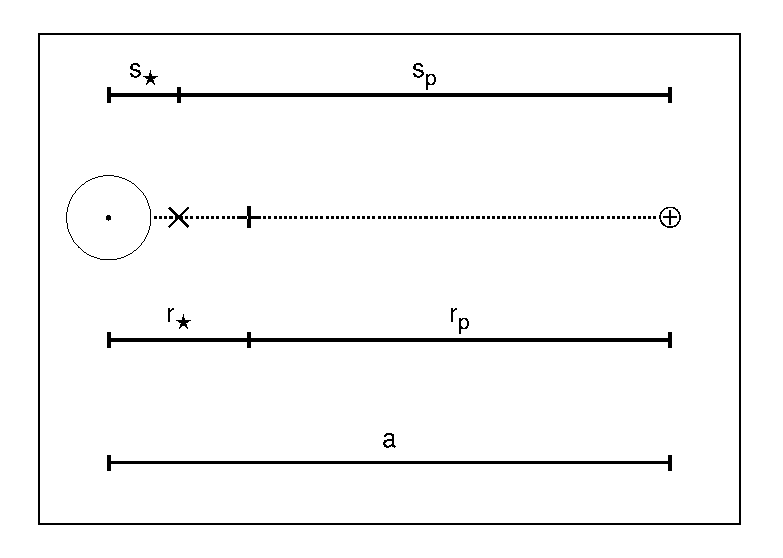
\epsfig{width=\linewidth,file=whalefig1.eps}
\caption[Whales are Everywhere (short caption example)]{An illustration of a system containing a star, shown on the left, and a whale, shown on the right, separated by a distance $a$, not to scale. The star and whale lie at distances of $r_{\star}$ and $r_{p}$, respectively, from the barycenter of the system, which is marked via a ``+'' symbol. Similarly, the star and whale lie at distances of $s_{\star}$ and $s_{p}$, respectively, from the photocenter of the system, which is marked via a ``$\times$'' symbol. All distances are sky-projected distances along the semi-major axis of the system, and thus are independent of the system's inclination. Note that although in this illustration the photocenter is to the left of the barycenter, it can lie anywhere between the star and whale.}
\label{whalefig1}
\end{figure}

\begin{figure}[h]  % Adding [h] will tell latex to place the figure with text if it can and looks good. If it can't place it with text (too big), then it goes to the end of the chapter and you will have to go back to [] or []h!]
\centering
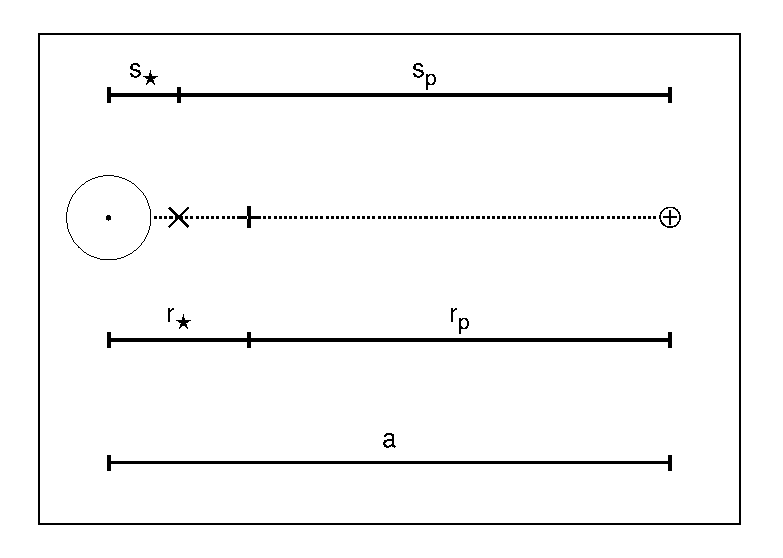
\epsfig{width=\linewidth,file=whalefig1.eps}
\caption[Whales are Everywhere (short caption example)]{An illustration of a system containing a star, shown on the left, and a whale, shown on the right, separated by a distance $a$, not to scale. The star and whale lie at distances of $r_{\star}$ and $r_{p}$, respectively, from the barycenter of the system, which is marked via a ``+'' symbol. Similarly, the star and whale lie at distances of $s_{\star}$ and $s_{p}$, respectively, from the photocenter of the system, which is marked via a ``$\times$'' symbol. All distances are sky-projected distances along the semi-major axis of the system, and thus are independent of the system's inclination. Note that although in this illustration the photocenter is to the left of the barycenter, it can lie anywhere between the star and whale.}
\label{whalefig1a}
\end{figure}

\begin{figure}[h!]  % Using [h!] will force it to go right here in the text, and be mroe aggressive about fitting text on the same page.
\centering
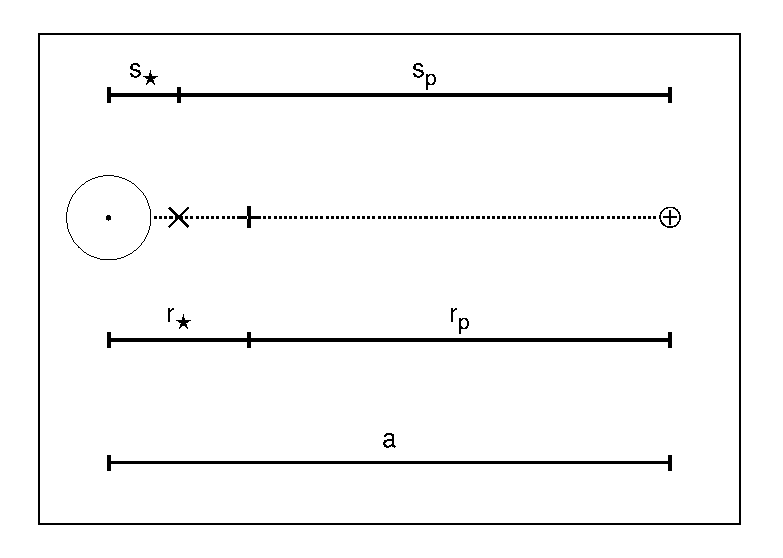
\epsfig{width=\linewidth,file=whalefig1.eps}
\caption[Whales are Everywhere (short caption example)]{An illustration of a system containing a star, shown on the left, and a whale, shown on the right, separated by a distance $a$, not to scale. The star and whale lie at distances of $r_{\star}$ and $r_{p}$, respectively, from the barycenter of the system, which is marked via a ``+'' symbol. Similarly, the star and whale lie at distances of $s_{\star}$ and $s_{p}$, respectively, from the photocenter of the system, which is marked via a ``$\times$'' symbol. All distances are sky-projected distances along the semi-major axis of the system, and thus are independent of the system's inclination. Note that although in this illustration the photocenter is to the left of the barycenter, it can lie anywhere between the star and whale.}
\label{whalefig1b}
\end{figure}

\tabletypesize{\scriptsize}
\begin{deluxetable}{ccccccccc}
  \tablewidth{0pt}
  \tablecaption{Currently Known Exoplanets with the Most Negative $\alpha_{WHALE}$ Values}
  \tablecolumns{9}
  \tablehead{Name & $D$ & $M_{\star}$ & $R_{\star}$ & $T_{\star}$ & $M_{p}$ & $R_{p}$ & $P$ & $\alpha_{WHALE}$ \\ & (pc) & (M$_{\sun}$) & (R$_{\sun}$) & (K) & (M$_{\rm J}$) & (R$_{\rm J}$) & (Days) & ($\mu$as)}
  \startdata
  \cutinhead{K Band (2.19 $\mu$m)}
  WASP-12 b & 427 & 1.28 & 1.63 & 6300 & 1.35 & 1.79 & 1.091 & -0.05 \\ 
WASP-19 b & 250 & 0.93 & 0.99 & 5500 & 1.11 & 1.39 & 0.789 & -0.05 \\ 
WASP-33 b & 115 & 1.50 & 1.44 & 7430 & 2.05 & 1.50 & 1.220 & -0.04 \\ 
55 Cnc e & 12 & 0.96 & 0.96 & 5234 & 0.03 & 0.19 & 0.737 & -0.01 \\ 
CoRoT-1 b & 480 & 0.95 & 1.11 & 5950 & 1.03 & 1.49 & 1.509 & -0.01 \\

  \cutinhead{L Band (3.45 $\mu$m)}
  HD 209458 b & 49 & 1.13 & 1.16 & 6065 & 0.69 & 1.36 & 3.525 & -0.23 \\ 
WASP-33 b & 115 & 1.50 & 1.44 & 7430 & 2.05 & 1.50 & 1.220 & -0.20 \\ 
WASP-19 b & 250 & 0.93 & 0.99 & 5500 & 1.11 & 1.39 & 0.789 & -0.15 \\ 
WASP-17 b & 300 & 1.19 & 1.20 & 6550 & 0.49 & 1.51 & 3.735 & -0.11 \\ 
WASP-12 b & 427 & 1.28 & 1.63 & 6300 & 1.35 & 1.79 & 1.091 & -0.10 \\ 

  \cutinhead{M Band (4.75 $\mu$m)}
  HD 209458 b & 49 & 1.13 & 1.16 & 6065 & 0.69 & 1.36 & 3.525 & -0.66 \\ 
HD 189733 b & 19 & 0.81 & 0.76 & 5040 & 1.14 & 1.14 & 2.219 & -0.47 \\ 
WASP-33 b & 115 & 1.50 & 1.44 & 7430 & 2.05 & 1.50 & 1.220 & -0.29 \\ 
WASP-19 b & 250 & 0.93 & 0.99 & 5500 & 1.11 & 1.39 & 0.789 & -0.21 \\ 
WASP-17 b & 300 & 1.19 & 1.20 & 6550 & 0.49 & 1.51 & 3.735 & -0.19 \\ 

  \cutinhead{N Band (10.0 $\mu$m)}
  HD 189733 b & 19 & 0.81 & 0.76 & 5040 & 1.14 & 1.14 & 2.219 & -3.04 \\ 
HD 209458 b & 49 & 1.13 & 1.16 & 6065 & 0.69 & 1.36 & 3.525 & -1.53 \\ 
Gliese 436 b & 10 & 0.45 & 0.46 & 3684 & 0.07 & 0.38 & 2.644 & -0.95 \\ 
WASP-34 b & 120 & 1.01 & 0.93 & 5700 & 0.58 & 1.22 & 4.318 & -0.64 \\ 
GJ 1214 b & 12 & 0.16 & 0.21 & 3026 & 0.02 & 0.24 & 1.580 & -0.59 

  \enddata
  \label{tab1}
\end{deluxetable}

\section{Further Whale Observations}

We get into detail about exowhales.

\subsection{Whales and You: What you Need to Know}

A subsection on whales and you.

\subsubsection{Whales: The Noisy Killer}

Everyone can hear you scream underwater.

\paragraph{Whale Colors}

A paragraph, (what you might want to label a subsubsubsection), and whale chromotography. We could go as deep in sections as a subparagraph, but, well, let's not.

Instead let's show a rotated deluxetable on whales with errorbars in Table~\ref{modelresultstab}.

\begin{deluxetable}{rcccccccccc}
  \rotate  % Comment out for portrait, leave uncommented for landscape
  \tablewidth{0pt}  % Gotta have this in every deluxetable
  \tabletypesize{\scriptsize}
%   \setlength{\tabcolsep}{5pt} % ONLY INCLUDE THIS LINE IF YOU NEED IT! Having it included squeezs column space slightly (smaller pt = tigheter tables) to make it fit in margins since its such a big table.
  \tablecaption{Modeling Results: Median Values and Associated 1$\sigma$ Uncertainties}
  \tablecolumns{11}
  \tablehead{KOI & $J$ & $r_{\rm sum}$ & $k$ & $i$ & $e$cos$w$ & $e$sin$w$ & $P$ & $T_{0}$ & $A_{L_{p}}$ & $\chi^{2}_{red}$\\ & & & & ($\degr$) & & & (Days) & (BJD-2450000) & & }
  \startdata
  \cutinhead{PDC Light Curve With Eccentricity Fixed to Zero}
     2.01 & $ $ 0.0108$^{_{+0.0013}}_{^{-0.0011}}$ & 0.254$^{_{+0.005}}_{^{-0.005}}$ & 0.0769$^{_{+0.0004}}_{^{-0.0004}}$ & 83.92$^{_{+0.7045}}_{^{-0.5848}}$ & $ $ 0.000$^{_{+0.000}}_{^{-0.000}}$ & $ $ 0.000$^{_{+0.000}}_{^{-0.000}}$ & 2.204732$^{_{+3.1\textrm{e-}06}}_{^{-3.0\textrm{e-}06}}$ & 4954.35796$^{_{+0.00013}}_{^{-0.00013}}$ & $ $ 0.421$^{_{+0.07}}_{^{-0.07}}$ & 26.5\\
   5.01 & $ $-0.0088$^{_{+0.0088}}_{^{-0.0097}}$ & 0.123$^{_{+0.010}}_{^{-0.013}}$ & 0.0356$^{_{+0.0009}}_{^{-0.0011}}$ & 83.60$^{_{+0.7978}}_{^{-0.5911}}$ & $ $ 0.000$^{_{+0.000}}_{^{-0.000}}$ & $ $ 0.000$^{_{+0.000}}_{^{-0.000}}$ & 4.780381$^{_{+6.7\textrm{e-}05}}_{^{-6.7\textrm{e-}05}}$ & 4965.97227$^{_{+0.00119}}_{^{-0.00121}}$ & $ $ 0.300$^{_{+0.72}}_{^{-0.35}}$ & 2.69\\
  10.01 & $ $ 0.0014$^{_{+0.0033}}_{^{-0.0013}}$ & 0.151$^{_{+0.004}}_{^{-0.004}}$ & 0.0938$^{_{+0.0006}}_{^{-0.0007}}$ & 84.68$^{_{+0.3495}}_{^{-0.2975}}$ & $ $ 0.000$^{_{+0.000}}_{^{-0.000}}$ & $ $ 0.000$^{_{+0.000}}_{^{-0.000}}$ & 3.522511$^{_{+1.5\textrm{e-}05}}_{^{-1.6\textrm{e-}05}}$ & 4954.11838$^{_{+0.00043}}_{^{-0.00041}}$ & $ $-5.752$^{_{+4.04}}_{^{-64.5}}$ & 4.31\\
  13.01 & $ $ 0.0248$^{_{+0.0013}}_{^{-0.0015}}$ & 0.294$^{_{+0.005}}_{^{-0.006}}$ & 0.0659$^{_{+0.0002}}_{^{-0.0003}}$ & 79.79$^{_{+0.5070}}_{^{-0.4079}}$ & $ $ 0.000$^{_{+0.000}}_{^{-0.000}}$ & $ $ 0.000$^{_{+0.000}}_{^{-0.000}}$ & 1.763589$^{_{+2.3\textrm{e-}06}}_{^{-2.3\textrm{e-}06}}$ & 4953.56510$^{_{+0.00013}}_{^{-0.00014}}$ & $ $ 0.339$^{_{+0.02}}_{^{-0.02}}$ & 15.9\\
  18.01 & $ $ 0.0000$^{_{+0.0001}}_{^{-0.0000}}$ & 0.174$^{_{+0.027}}_{^{-0.005}}$ & 0.0783$^{_{+0.0025}}_{^{-0.0007}}$ & 87.64$^{_{+1.7674}}_{^{-3.6176}}$ & $ $ 0.000$^{_{+0.000}}_{^{-0.000}}$ & $ $ 0.000$^{_{+0.000}}_{^{-0.000}}$ & 3.548460$^{_{+2.4\textrm{e-}05}}_{^{-2.5\textrm{e-}05}}$ & 4955.90081$^{_{+0.00068}}_{^{-0.00064}}$ & $ $-78.785$^{_{+238.}}_{^{-525.}}$ & 9.33\\
  64.01 & $ $ 0.0207$^{_{+0.0104}}_{^{-0.0100}}$ & 0.283$^{_{+0.018}}_{^{-0.019}}$ & 0.0425$^{_{+0.0018}}_{^{-0.0013}}$ & 75.01$^{_{+1.1206}}_{^{-1.0527}}$ & $ $ 0.000$^{_{+0.000}}_{^{-0.000}}$ & $ $ 0.000$^{_{+0.000}}_{^{-0.000}}$ & 1.951178$^{_{+2.8\textrm{e-}05}}_{^{-2.9\textrm{e-}05}}$ & 4990.53822$^{_{+0.00086}}_{^{-0.00086}}$ & $ $-0.312$^{_{+0.62}}_{^{-0.84}}$ & 10.4\\
  97.01 & $ $ 0.0066$^{_{+0.0017}}_{^{-0.0016}}$ & 0.156$^{_{+0.003}}_{^{-0.004}}$ & 0.0817$^{_{+0.0005}}_{^{-0.0005}}$ & 85.93$^{_{+0.4176}}_{^{-0.3637}}$ & $ $ 0.000$^{_{+0.000}}_{^{-0.000}}$ & $ $ 0.000$^{_{+0.000}}_{^{-0.000}}$ & 4.885495$^{_{+1.7\textrm{e-}05}}_{^{-1.7\textrm{e-}05}}$ & 4967.27590$^{_{+0.00030}}_{^{-0.00031}}$ & $ $ 0.115$^{_{+0.24}}_{^{-0.23}}$ & 2.24\\
 102.01 & $ $ 0.0140$^{_{+0.0089}}_{^{-0.0101}}$ & 0.199$^{_{+0.026}}_{^{-0.021}}$ & 0.0284$^{_{+0.0008}}_{^{-0.0007}}$ & 84.17$^{_{+2.8540}}_{^{-2.5667}}$ & $ $ 0.000$^{_{+0.000}}_{^{-0.000}}$ & $ $ 0.000$^{_{+0.000}}_{^{-0.000}}$ & 1.735114$^{_{+2.1\textrm{e-}05}}_{^{-2.1\textrm{e-}05}}$ & 4968.06072$^{_{+0.00101}}_{^{-0.00102}}$ & $ $-0.187$^{_{+0.34}}_{^{-0.56}}$ & 2.32\\
 144.01 & $ $ 0.0353$^{_{+0.0337}}_{^{-0.0292}}$ & 0.127$^{_{+0.026}}_{^{-0.012}}$ & 0.0352$^{_{+0.0021}}_{^{-0.0012}}$ & 86.86$^{_{+2.3598}}_{^{-2.5586}}$ & $ $ 0.000$^{_{+0.000}}_{^{-0.000}}$ & $ $ 0.000$^{_{+0.000}}_{^{-0.000}}$ & 4.176149$^{_{+1.5\textrm{e-}04}}_{^{-1.6\textrm{e-}04}}$ & 4966.09112$^{_{+0.00322}}_{^{-0.00310}}$ & $ $ 2.019$^{_{+5.88}}_{^{-1.25}}$ & 6.92\\
 186.01 & $ $-0.0014$^{_{+0.0026}}_{^{-0.0027}}$ & 0.126$^{_{+0.005}}_{^{-0.003}}$ & 0.1218$^{_{+0.0011}}_{^{-0.0008}}$ & 88.51$^{_{+1.3964}}_{^{-0.8215}}$ & $ $ 0.000$^{_{+0.000}}_{^{-0.000}}$ & $ $ 0.000$^{_{+0.000}}_{^{-0.000}}$ & 3.243268$^{_{+1.3\textrm{e-}05}}_{^{-1.4\textrm{e-}05}}$ & 4966.66796$^{_{+0.00037}}_{^{-0.00036}}$ & $ $ 0.051$^{_{+0.93}}_{^{-1.12}}$ & 3.20\\
 188.01 & $ $ 0.0033$^{_{+0.0024}}_{^{-0.0022}}$ & 0.092$^{_{+0.004}}_{^{-0.004}}$ & 0.1155$^{_{+0.0016}}_{^{-0.0018}}$ & 87.37$^{_{+0.4475}}_{^{-0.3527}}$ & $ $ 0.000$^{_{+0.000}}_{^{-0.000}}$ & $ $ 0.000$^{_{+0.000}}_{^{-0.000}}$ & 3.797023$^{_{+1.2\textrm{e-}05}}_{^{-1.2\textrm{e-}05}}$ & 4966.50793$^{_{+0.00029}}_{^{-0.00028}}$ & $ $-0.309$^{_{+0.43}}_{^{-0.68}}$ & 2.14\\
 195.01 & $ $ 0.0047$^{_{+0.0027}}_{^{-0.0030}}$ & 0.107$^{_{+0.004}}_{^{-0.004}}$ & 0.1165$^{_{+0.0011}}_{^{-0.0013}}$ & 86.42$^{_{+0.3423}}_{^{-0.2949}}$ & $ $ 0.000$^{_{+0.000}}_{^{-0.000}}$ & $ $ 0.000$^{_{+0.000}}_{^{-0.000}}$ & 3.217522$^{_{+1.2\textrm{e-}05}}_{^{-1.3\textrm{e-}05}}$ & 4966.63096$^{_{+0.00033}}_{^{-0.00032}}$ & $ $-0.132$^{_{+0.42}}_{^{-0.56}}$ & 2.38\\
 196.01 & $ $ 0.0060$^{_{+0.0019}}_{^{-0.0019}}$ & 0.221$^{_{+0.005}}_{^{-0.006}}$ & 0.1022$^{_{+0.0007}}_{^{-0.0008}}$ & 82.05$^{_{+0.4642}}_{^{-0.3994}}$ & $ $ 0.000$^{_{+0.000}}_{^{-0.000}}$ & $ $ 0.000$^{_{+0.000}}_{^{-0.000}}$ & 1.855561$^{_{+5.0\textrm{e-}06}}_{^{-5.4\textrm{e-}06}}$ & 4970.18013$^{_{+0.00024}}_{^{-0.00023}}$ & $ $-0.168$^{_{+0.19}}_{^{-0.25}}$ & 2.33\\
 199.01 & $ $ 0.0029$^{_{+0.0030}}_{^{-0.0032}}$ & 0.151$^{_{+0.006}}_{^{-0.007}}$ & 0.0963$^{_{+0.0009}}_{^{-0.0009}}$ & 86.81$^{_{+1.0287}}_{^{-0.7643}}$ & $ $ 0.000$^{_{+0.000}}_{^{-0.000}}$ & $ $ 0.000$^{_{+0.000}}_{^{-0.000}}$ & 3.268695$^{_{+1.7\textrm{e-}05}}_{^{-1.6\textrm{e-}05}}$ & 4970.48096$^{_{+0.00043}}_{^{-0.00044}}$ & $ $ 0.079$^{_{+0.41}}_{^{-0.44}}$ & 1.40\\
 201.01 & $ $-0.0059$^{_{+0.0051}}_{^{-0.0051}}$ & 0.093$^{_{+0.009}}_{^{-0.005}}$ & 0.0800$^{_{+0.0021}}_{^{-0.0012}}$ & 88.31$^{_{+1.5193}}_{^{-1.1075}}$ & $ $ 0.000$^{_{+0.000}}_{^{-0.000}}$ & $ $ 0.000$^{_{+0.000}}_{^{-0.000}}$ & 4.225373$^{_{+2.1\textrm{e-}05}}_{^{-2.2\textrm{e-}05}}$ & 4970.56037$^{_{+0.00039}}_{^{-0.00039}}$ & $ $ 1.145$^{_{+1.92}}_{^{-0.81}}$ & 3.60\\
 202.01 & $ $ 0.0053$^{_{+0.0023}}_{^{-0.0023}}$ & 0.225$^{_{+0.004}}_{^{-0.004}}$ & 0.1040$^{_{+0.0006}}_{^{-0.0006}}$ & 80.75$^{_{+0.2992}}_{^{-0.2744}}$ & $ $ 0.000$^{_{+0.000}}_{^{-0.000}}$ & $ $ 0.000$^{_{+0.000}}_{^{-0.000}}$ & 1.720867$^{_{+4.4\textrm{e-}06}}_{^{-4.7\textrm{e-}06}}$ & 4966.02007$^{_{+0.00023}}_{^{-0.00023}}$ & $ $-0.333$^{_{+0.22}}_{^{-0.38}}$ & 8.81\\
 204.01 & $ $-0.0019$^{_{+0.0032}}_{^{-0.0041}}$ & 0.151$^{_{+0.012}}_{^{-0.014}}$ & 0.0817$^{_{+0.0017}}_{^{-0.0022}}$ & 85.16$^{_{+1.4103}}_{^{-0.9589}}$ & $ $ 0.000$^{_{+0.000}}_{^{-0.000}}$ & $ $ 0.000$^{_{+0.000}}_{^{-0.000}}$ & 3.246708$^{_{+2.4\textrm{e-}05}}_{^{-2.6\textrm{e-}05}}$ & 4966.37897$^{_{+0.00067}}_{^{-0.00064}}$ & $ $ 1.579$^{_{+6.48}}_{^{-3.05}}$ & 2.08\\
 229.01 & $ $ 0.0000$^{_{+0.0004}}_{^{-0.0000}}$ & 0.400$^{_{+0.005}}_{^{-0.005}}$ & 0.2872$^{_{+0.0327}}_{^{-0.0289}}$ & 67.77$^{_{+0.3073}}_{^{-0.3087}}$ & $ $ 0.000$^{_{+0.000}}_{^{-0.000}}$ & $ $ 0.000$^{_{+0.000}}_{^{-0.000}}$ & 3.573190$^{_{+8.5\textrm{e-}05}}_{^{-8.7\textrm{e-}05}}$ & 4967.93368$^{_{+0.00196}}_{^{-0.00200}}$ & $ $-2.565$^{_{+3.04}}_{^{-27.4}}$ & 1.98\\
 356.01 & $ $ 0.0007$^{_{+0.0140}}_{^{-0.0115}}$ & 0.169$^{_{+0.055}}_{^{-0.026}}$ & 0.0334$^{_{+0.0026}}_{^{-0.0013}}$ & 84.64$^{_{+3.6556}}_{^{-4.5146}}$ & $ $ 0.000$^{_{+0.000}}_{^{-0.000}}$ & $ $ 0.000$^{_{+0.000}}_{^{-0.000}}$ & 1.827099$^{_{+3.1\textrm{e-}05}}_{^{-3.2\textrm{e-}05}}$ & 5003.52457$^{_{+0.00093}}_{^{-0.00093}}$ & $ $-0.007$^{_{+0.81}}_{^{-1.10}}$ & 1.52\\
 412.01 & $ $ 0.0063$^{_{+0.0116}}_{^{-0.0121}}$ & 0.100$^{_{+0.025}}_{^{-0.008}}$ & 0.0571$^{_{+0.0030}}_{^{-0.0012}}$ & 87.79$^{_{+1.7520}}_{^{-2.3886}}$ & $ $ 0.000$^{_{+0.000}}_{^{-0.000}}$ & $ $ 0.000$^{_{+0.000}}_{^{-0.000}}$ & 4.146994$^{_{+5.6\textrm{e-}05}}_{^{-5.7\textrm{e-}05}}$ & 5003.32536$^{_{+0.00073}}_{^{-0.00075}}$ & $ $-0.487$^{_{+1.49}}_{^{-2.00}}$ & 2.64\\
 421.01 & $ $-0.0059$^{_{+0.0048}}_{^{-0.0042}}$ & 0.076$^{_{+0.005}}_{^{-0.005}}$ & 0.1197$^{_{+0.0021}}_{^{-0.0024}}$ & 88.00$^{_{+0.5723}}_{^{-0.4216}}$ & $ $ 0.000$^{_{+0.000}}_{^{-0.000}}$ & $ $ 0.000$^{_{+0.000}}_{^{-0.000}}$ & 4.454225$^{_{+2.2\textrm{e-}05}}_{^{-2.3\textrm{e-}05}}$ & 5005.81890$^{_{+0.00028}}_{^{-0.00026}}$ & $ $ 0.137$^{_{+0.83}}_{^{-0.72}}$ & 4.01\\
 433.01 & $ $ 0.0001$^{_{+0.0162}}_{^{-0.0202}}$ & 0.352$^{_{+0.055}}_{^{-0.070}}$ & 0.2406$^{_{+0.1861}}_{^{-0.1474}}$ & 70.78$^{_{+4.5618}}_{^{-3.4365}}$ & $ $ 0.000$^{_{+0.000}}_{^{-0.000}}$ & $ $ 0.000$^{_{+0.000}}_{^{-0.000}}$ & 4.030457$^{_{+1.5\textrm{e-}04}}_{^{-1.4\textrm{e-}04}}$ & 5004.09086$^{_{+0.00179}}_{^{-0.00180}}$ & $ $ 0.033$^{_{+0.56}}_{^{-0.10}}$ & 7.51\\
 611.01 & $ $-0.0030$^{_{+0.0078}}_{^{-0.0075}}$ & 0.126$^{_{+0.009}}_{^{-0.006}}$ & 0.0760$^{_{+0.0077}}_{^{-0.0022}}$ & 83.75$^{_{+0.3507}}_{^{-0.5390}}$ & $ $ 0.000$^{_{+0.000}}_{^{-0.000}}$ & $ $ 0.000$^{_{+0.000}}_{^{-0.000}}$ & 3.251646$^{_{+2.8\textrm{e-}05}}_{^{-2.6\textrm{e-}05}}$ & 5004.05985$^{_{+0.00038}}_{^{-0.00040}}$ & $ $-0.039$^{_{+0.73}}_{^{-0.74}}$ & 2.12\\
 684.01 & $ $ 0.0802$^{_{+0.0491}}_{^{-0.0439}}$ & 0.066$^{_{+0.028}}_{^{-0.016}}$ & 0.0269$^{_{+0.0029}}_{^{-0.0019}}$ & 87.36$^{_{+1.6669}}_{^{-2.0032}}$ & $ $ 0.000$^{_{+0.000}}_{^{-0.000}}$ & $ $ 0.000$^{_{+0.000}}_{^{-0.000}}$ & 4.035328$^{_{+1.9\textrm{e-}04}}_{^{-1.8\textrm{e-}04}}$ & 5005.25386$^{_{+0.00223}}_{^{-0.00229}}$ & $ $-0.183$^{_{+0.17}}_{^{-0.32}}$ & 2.11\\
 760.01 & $ $ 0.0023$^{_{+0.0054}}_{^{-0.0052}}$ & 0.094$^{_{+0.003}}_{^{-0.003}}$ & 0.1055$^{_{+0.0013}}_{^{-0.0013}}$ & 85.85$^{_{+0.1909}}_{^{-0.1787}}$ & $ $ 0.000$^{_{+0.000}}_{^{-0.000}}$ & $ $ 0.000$^{_{+0.000}}_{^{-0.000}}$ & 4.959343$^{_{+4.4\textrm{e-}05}}_{^{-4.4\textrm{e-}05}}$ & 5005.25676$^{_{+0.00043}}_{^{-0.00045}}$ & $ $-0.300$^{_{+1.14}}_{^{-1.38}}$ & 1.83\\
 801.01 & $ $ 0.0061$^{_{+0.0067}}_{^{-0.0059}}$ & 0.221$^{_{+0.021}}_{^{-0.023}}$ & 0.0865$^{_{+0.0023}}_{^{-0.0025}}$ & 83.93$^{_{+3.0796}}_{^{-1.9812}}$ & $ $ 0.000$^{_{+0.000}}_{^{-0.000}}$ & $ $ 0.000$^{_{+0.000}}_{^{-0.000}}$ & 1.625498$^{_{+1.1\textrm{e-}05}}_{^{-1.1\textrm{e-}05}}$ & 5003.82699$^{_{+0.00035}}_{^{-0.00037}}$ & $ $-0.722$^{_{+0.87}}_{^{-2.05}}$ & 2.81\\
 809.01 & $ $-0.0023$^{_{+0.0041}}_{^{-0.0048}}$ & 0.163$^{_{+0.017}}_{^{-0.007}}$ & 0.1177$^{_{+0.0027}}_{^{-0.0011}}$ & 87.56$^{_{+2.0953}}_{^{-2.2216}}$ & $ $ 0.000$^{_{+0.000}}_{^{-0.000}}$ & $ $ 0.000$^{_{+0.000}}_{^{-0.000}}$ & 1.594742$^{_{+7.1\textrm{e-}06}}_{^{-7.1\textrm{e-}06}}$ & 5003.64754$^{_{+0.00024}}_{^{-0.00023}}$ & $ $ 0.779$^{_{+2.22}}_{^{-2.24}}$ & 3.47\\
 813.01 & $ $-0.0166$^{_{+0.0094}}_{^{-0.0091}}$ & 0.089$^{_{+0.017}}_{^{-0.012}}$ & 0.0897$^{_{+0.0042}}_{^{-0.0031}}$ & 87.62$^{_{+2.2020}}_{^{-1.5063}}$ & $ $ 0.000$^{_{+0.000}}_{^{-0.000}}$ & $ $ 0.000$^{_{+0.000}}_{^{-0.000}}$ & 3.895887$^{_{+5.2\textrm{e-}05}}_{^{-5.4\textrm{e-}05}}$ & 5003.52771$^{_{+0.00069}}_{^{-0.00066}}$ & $ $-0.070$^{_{+0.34}}_{^{-0.42}}$ & 1.72\\
 830.01 & $ $ 0.0024$^{_{+0.0031}}_{^{-0.0032}}$ & 0.099$^{_{+0.006}}_{^{-0.002}}$ & 0.1370$^{_{+0.0026}}_{^{-0.0010}}$ & 89.03$^{_{+0.8555}}_{^{-1.0199}}$ & $ $ 0.000$^{_{+0.000}}_{^{-0.000}}$ & $ $ 0.000$^{_{+0.000}}_{^{-0.000}}$ & 3.525638$^{_{+1.1\textrm{e-}05}}_{^{-1.1\textrm{e-}05}}$ & 5003.04715$^{_{+0.00015}}_{^{-0.00015}}$ & $ $-0.775$^{_{+1.88}}_{^{-2.58}}$ & 4.23\\
 838.01 & $ $ 0.0001$^{_{+0.0044}}_{^{-0.0028}}$ & 0.118$^{_{+0.009}}_{^{-0.010}}$ & 0.1047$^{_{+0.0235}}_{^{-0.0139}}$ & 84.18$^{_{+0.5842}}_{^{-0.5591}}$ & $ $ 0.000$^{_{+0.000}}_{^{-0.000}}$ & $ $ 0.000$^{_{+0.000}}_{^{-0.000}}$ & 4.859423$^{_{+8.1\textrm{e-}05}}_{^{-8.2\textrm{e-}05}}$ & 5006.01042$^{_{+0.00077}}_{^{-0.00082}}$ & $ $ 1.279$^{_{+100.}}_{^{-18.1}}$ & 7.50\\
 840.01 & $ $-0.0045$^{_{+0.0061}}_{^{-0.0061}}$ & 0.113$^{_{+0.008}}_{^{-0.008}}$ & 0.1048$^{_{+0.0024}}_{^{-0.0026}}$ & 85.44$^{_{+0.5689}}_{^{-0.4960}}$ & $ $ 0.000$^{_{+0.000}}_{^{-0.000}}$ & $ $ 0.000$^{_{+0.000}}_{^{-0.000}}$ & 3.040348$^{_{+2.2\textrm{e-}05}}_{^{-2.3\textrm{e-}05}}$ & 5002.94813$^{_{+0.00041}}_{^{-0.00042}}$ & $ $ 0.104$^{_{+1.14}}_{^{-1.13}}$ & 4.10\\
 843.01 & $ $-0.0007$^{_{+0.0052}}_{^{-0.0135}}$ & 0.132$^{_{+0.027}}_{^{-0.032}}$ & 0.0544$^{_{+0.0028}}_{^{-0.0034}}$ & 84.60$^{_{+2.7198}}_{^{-1.8763}}$ & $ $ 0.000$^{_{+0.000}}_{^{-0.000}}$ & $ $ 0.000$^{_{+0.000}}_{^{-0.000}}$ & 4.190630$^{_{+1.1\textrm{e-}04}}_{^{-1.1\textrm{e-}04}}$ & 5004.43891$^{_{+0.00134}}_{^{-0.00137}}$ & $ $ 0.935$^{_{+61.1}}_{^{-2.33}}$ & 1.51\\
 897.01 & $ $ 0.0032$^{_{+0.0036}}_{^{-0.0032}}$ & 0.159$^{_{+0.008}}_{^{-0.010}}$ & 0.1166$^{_{+0.0016}}_{^{-0.0019}}$ & 85.30$^{_{+0.9264}}_{^{-0.7186}}$ & $ $ 0.000$^{_{+0.000}}_{^{-0.000}}$ & $ $ 0.000$^{_{+0.000}}_{^{-0.000}}$ & 2.052344$^{_{+8.8\textrm{e-}06}}_{^{-8.7\textrm{e-}06}}$ & 5002.89010$^{_{+0.00022}}_{^{-0.00022}}$ & $ $-1.469$^{_{+1.28}}_{^{-4.03}}$ & 2.58\\
 908.01 & $ $ 0.0050$^{_{+0.0060}}_{^{-0.0052}}$ & 0.092$^{_{+0.012}}_{^{-0.004}}$ & 0.0839$^{_{+0.0026}}_{^{-0.0010}}$ & 88.63$^{_{+1.2397}}_{^{-1.4946}}$ & $ $ 0.000$^{_{+0.000}}_{^{-0.000}}$ & $ $ 0.000$^{_{+0.000}}_{^{-0.000}}$ & 4.708363$^{_{+4.8\textrm{e-}05}}_{^{-4.8\textrm{e-}05}}$ & 5004.44523$^{_{+0.00048}}_{^{-0.00046}}$ & $ $ 0.200$^{_{+0.78}}_{^{-0.61}}$ & 1.47\\
 913.01 & $ $ 0.0021$^{_{+0.0027}}_{^{-0.0027}}$ & 0.105$^{_{+0.004}}_{^{-0.002}}$ & 0.1240$^{_{+0.0012}}_{^{-0.0007}}$ & 89.05$^{_{+0.8784}}_{^{-0.8239}}$ & $ $ 0.000$^{_{+0.000}}_{^{-0.000}}$ & $ $ 0.000$^{_{+0.000}}_{^{-0.000}}$ & 4.082286$^{_{+2.0\textrm{e-}05}}_{^{-1.9\textrm{e-}05}}$ & 5002.63669$^{_{+0.00023}}_{^{-0.00023}}$ & $ $ 0.162$^{_{+1.88}}_{^{-1.85}}$ & 2.82\\
 931.01 & $ $ 0.0007$^{_{+0.0034}}_{^{-0.0010}}$ & 0.112$^{_{+0.009}}_{^{-0.003}}$ & 0.1201$^{_{+0.0024}}_{^{-0.0008}}$ & 88.67$^{_{+1.0903}}_{^{-1.4164}}$ & $ $ 0.000$^{_{+0.000}}_{^{-0.000}}$ & $ $ 0.000$^{_{+0.000}}_{^{-0.000}}$ & 3.855646$^{_{+2.3\textrm{e-}05}}_{^{-2.2\textrm{e-}05}}$ & 5003.67760$^{_{+0.00028}}_{^{-0.00030}}$ & $ $-2.995$^{_{+6.90}}_{^{-45.3}}$ & 2.63\\
 961.02 & $ $ 0.0017$^{_{+0.0198}}_{^{-0.0184}}$ & 0.292$^{_{+0.076}}_{^{-0.072}}$ & 0.0486$^{_{+0.0108}}_{^{-0.0050}}$ & 75.39$^{_{+4.6244}}_{^{-4.8234}}$ & $ $ 0.000$^{_{+0.000}}_{^{-0.000}}$ & $ $ 0.000$^{_{+0.000}}_{^{-0.000}}$ & 0.453296$^{_{+6.3\textrm{e-}06}}_{^{-6.3\textrm{e-}06}}$ & 4966.86709$^{_{+0.00116}}_{^{-0.00114}}$ & $ $ 0.048$^{_{+0.32}}_{^{-0.34}}$ & 1.95\\
 961.03 & $ $ 0.0159$^{_{+0.0472}}_{^{-0.0397}}$ & 0.060$^{_{+0.004}}_{^{-0.004}}$ & 0.4879$^{_{+1.0011}}_{^{-0.4024}}$ & 86.69$^{_{+0.2489}}_{^{-0.2260}}$ & $ $ 0.000$^{_{+0.000}}_{^{-0.000}}$ & $ $ 0.000$^{_{+0.000}}_{^{-0.000}}$ & 1.865033$^{_{+5.5\textrm{e-}05}}_{^{-5.8\textrm{e-}05}}$ & 4966.79647$^{_{+0.00259}}_{^{-0.00251}}$ & $ $ 0.000$^{_{+0.00}}_{^{-0.00}}$ & 2.30\\
1419.01 & $ $ 0.0131$^{_{+0.0145}}_{^{-0.0130}}$ & 0.322$^{_{+0.049}}_{^{-0.050}}$ & 0.0555$^{_{+0.0128}}_{^{-0.0034}}$ & 73.38$^{_{+3.0786}}_{^{-3.1111}}$ & $ $ 0.000$^{_{+0.000}}_{^{-0.000}}$ & $ $ 0.000$^{_{+0.000}}_{^{-0.000}}$ & 1.336074$^{_{+2.7\textrm{e-}05}}_{^{-2.8\textrm{e-}05}}$ & 5011.25875$^{_{+0.00087}}_{^{-0.00092}}$ & $ $-0.874$^{_{+0.85}}_{^{-2.18}}$ & 1.99\\
1459.01 & $ $ 0.0267$^{_{+0.0110}}_{^{-0.0127}}$ & 0.403$^{_{+0.044}}_{^{-0.061}}$ & 0.0930$^{_{+0.0367}}_{^{-0.0143}}$ & 69.77$^{_{+4.0056}}_{^{-3.0350}}$ & $ $ 0.000$^{_{+0.000}}_{^{-0.000}}$ & $ $ 0.000$^{_{+0.000}}_{^{-0.000}}$ & 0.692024$^{_{+7.7\textrm{e-}06}}_{^{-7.2\textrm{e-}06}}$ & 4966.11024$^{_{+0.00088}}_{^{-0.00092}}$ & $ $ 1.794$^{_{+1.71}}_{^{-0.97}}$ & 9.55\\

  \cutinhead{CLM Light Curve With Eccentricity Fixed to Zero}
     1.01 & $ $-0.0002$^{_{+0.0004}}_{^{-0.0004}}$ & 0.142$^{_{+0.000}}_{^{-0.000}}$ & 0.1250$^{_{+0.0002}}_{^{-0.0002}}$ & 83.90$^{_{+0.0307}}_{^{-0.0291}}$ & $ $ 0.000$^{_{+0.000}}_{^{-0.000}}$ & $ $ 0.000$^{_{+0.000}}_{^{-0.000}}$ & 2.470614$^{_{+1.3\textrm{e-}06}}_{^{-1.3\textrm{e-}06}}$ & 4955.76254$^{_{+0.00005}}_{^{-0.00005}}$ & $ $ 0.250$^{_{+0.80}}_{^{-0.80}}$ & 1.94\\
   2.01 & $ $ 0.0113$^{_{+0.0014}}_{^{-0.0013}}$ & 0.255$^{_{+0.005}}_{^{-0.005}}$ & 0.0766$^{_{+0.0004}}_{^{-0.0004}}$ & 83.74$^{_{+0.6427}}_{^{-0.5590}}$ & $ $ 0.000$^{_{+0.000}}_{^{-0.000}}$ & $ $ 0.000$^{_{+0.000}}_{^{-0.000}}$ & 2.204733$^{_{+3.1\textrm{e-}06}}_{^{-3.0\textrm{e-}06}}$ & 4954.35793$^{_{+0.00013}}_{^{-0.00014}}$ & $ $ 0.240$^{_{+0.06}}_{^{-0.04}}$ & 7.61\\
   5.01 & $ $-0.0021$^{_{+0.0079}}_{^{-0.0087}}$ & 0.114$^{_{+0.012}}_{^{-0.016}}$ & 0.0354$^{_{+0.0011}}_{^{-0.0013}}$ & 84.15$^{_{+0.9448}}_{^{-0.7226}}$ & $ $ 0.000$^{_{+0.000}}_{^{-0.000}}$ & $ $ 0.000$^{_{+0.000}}_{^{-0.000}}$ & 4.780406$^{_{+6.8\textrm{e-}05}}_{^{-7.0\textrm{e-}05}}$ & 4965.97184$^{_{+0.00120}}_{^{-0.00121}}$ & $ $ 0.238$^{_{+0.92}}_{^{-0.92}}$ & 2.08\\
  10.01 & $ $ 0.0019$^{_{+0.0030}}_{^{-0.0032}}$ & 0.159$^{_{+0.005}}_{^{-0.005}}$ & 0.0929$^{_{+0.0007}}_{^{-0.0007}}$ & 84.11$^{_{+0.3818}}_{^{-0.3455}}$ & $ $ 0.000$^{_{+0.000}}_{^{-0.000}}$ & $ $ 0.000$^{_{+0.000}}_{^{-0.000}}$ & 3.522496$^{_{+1.9\textrm{e-}05}}_{^{-1.9\textrm{e-}05}}$ & 4954.11867$^{_{+0.00052}}_{^{-0.00053}}$ & $ $-1.296$^{_{+2.76}}_{^{-4.42}}$ & 2.71\\
  13.01 & $ $ 0.0253$^{_{+0.0012}}_{^{-0.0016}}$ & 0.287$^{_{+0.005}}_{^{-0.005}}$ & 0.0656$^{_{+0.0002}}_{^{-0.0003}}$ & 80.36$^{_{+0.4700}}_{^{-0.4390}}$ & $ $ 0.000$^{_{+0.000}}_{^{-0.000}}$ & $ $ 0.000$^{_{+0.000}}_{^{-0.000}}$ & 1.763585$^{_{+1.6\textrm{e-}06}}_{^{-1.7\textrm{e-}06}}$ & 4953.56529$^{_{+0.00008}}_{^{-0.00009}}$ & $ $ 0.286$^{_{+0.02}}_{^{-0.01}}$ & 3.89\\
  17.01 & $ $-0.0015$^{_{+0.0015}}_{^{-0.0019}}$ & 0.165$^{_{+0.005}}_{^{-0.006}}$ & 0.0955$^{_{+0.0008}}_{^{-0.0009}}$ & 85.73$^{_{+0.6314}}_{^{-0.5396}}$ & $ $ 0.000$^{_{+0.000}}_{^{-0.000}}$ & $ $ 0.000$^{_{+0.000}}_{^{-0.000}}$ & 3.234699$^{_{+1.2\textrm{e-}05}}_{^{-1.2\textrm{e-}05}}$ & 4954.48575$^{_{+0.00035}}_{^{-0.00036}}$ & $ $ 1.249$^{_{+3.52}}_{^{-1.93}}$ & 2.65\\
  18.01 & $ $-0.0037$^{_{+0.0040}}_{^{-0.0044}}$ & 0.173$^{_{+0.016}}_{^{-0.004}}$ & 0.0771$^{_{+0.0015}}_{^{-0.0005}}$ & 87.86$^{_{+1.6741}}_{^{-2.5008}}$ & $ $ 0.000$^{_{+0.000}}_{^{-0.000}}$ & $ $ 0.000$^{_{+0.000}}_{^{-0.000}}$ & 3.548447$^{_{+2.6\textrm{e-}05}}_{^{-2.7\textrm{e-}05}}$ & 4955.90128$^{_{+0.00074}}_{^{-0.00072}}$ & $ $ 1.457$^{_{+2.51}}_{^{-3.06}}$ & 3.73\\
  20.01 & $ $ 0.0003$^{_{+0.0010}}_{^{-0.0005}}$ & 0.142$^{_{+0.002}}_{^{-0.002}}$ & 0.1174$^{_{+0.0005}}_{^{-0.0005}}$ & 88.17$^{_{+0.5236}}_{^{-0.4041}}$ & $ $ 0.000$^{_{+0.000}}_{^{-0.000}}$ & $ $ 0.000$^{_{+0.000}}_{^{-0.000}}$ & 4.437979$^{_{+1.1\textrm{e-}05}}_{^{-1.0\textrm{e-}05}}$ & 5004.00819$^{_{+0.00011}}_{^{-0.00011}}$ & $ $-2.544$^{_{+4.51}}_{^{-30.3}}$ & 1.57\\
  64.01 & $ $ 0.0312$^{_{+0.0117}}_{^{-0.0112}}$ & 0.304$^{_{+0.028}}_{^{-0.019}}$ & 0.0427$^{_{+0.0050}}_{^{-0.0014}}$ & 73.80$^{_{+1.1307}}_{^{-1.7207}}$ & $ $ 0.000$^{_{+0.000}}_{^{-0.000}}$ & $ $ 0.000$^{_{+0.000}}_{^{-0.000}}$ & 1.951144$^{_{+3.3\textrm{e-}05}}_{^{-3.5\textrm{e-}05}}$ & 4990.53863$^{_{+0.00112}}_{^{-0.00109}}$ & $ $-0.120$^{_{+0.39}}_{^{-0.51}}$ & 7.24\\
  97.01 & $ $ 0.0084$^{_{+0.0022}}_{^{-0.0022}}$ & 0.154$^{_{+0.004}}_{^{-0.004}}$ & 0.0808$^{_{+0.0005}}_{^{-0.0006}}$ & 86.17$^{_{+0.5356}}_{^{-0.4202}}$ & $ $ 0.000$^{_{+0.000}}_{^{-0.000}}$ & $ $ 0.000$^{_{+0.000}}_{^{-0.000}}$ & 4.885522$^{_{+2.0\textrm{e-}05}}_{^{-2.0\textrm{e-}05}}$ & 4967.27550$^{_{+0.00034}}_{^{-0.00034}}$ & $ $-0.174$^{_{+0.06}}_{^{-0.09}}$ & 2.06\\
 127.01 & $ $-0.0026$^{_{+0.0031}}_{^{-0.0037}}$ & 0.117$^{_{+0.008}}_{^{-0.008}}$ & 0.0982$^{_{+0.0018}}_{^{-0.0018}}$ & 87.45$^{_{+1.3596}}_{^{-0.9077}}$ & $ $ 0.000$^{_{+0.000}}_{^{-0.000}}$ & $ $ 0.000$^{_{+0.000}}_{^{-0.000}}$ & 3.578772$^{_{+2.1\textrm{e-}05}}_{^{-2.1\textrm{e-}05}}$ & 4967.02976$^{_{+0.00048}}_{^{-0.00048}}$ & $ $ 0.151$^{_{+0.87}}_{^{-0.93}}$ & 3.80\\
 128.01 & $ $-0.0007$^{_{+0.0006}}_{^{-0.0029}}$ & 0.116$^{_{+0.003}}_{^{-0.003}}$ & 0.0983$^{_{+0.0007}}_{^{-0.0008}}$ & 85.73$^{_{+0.2412}}_{^{-0.2261}}$ & $ $ 0.000$^{_{+0.000}}_{^{-0.000}}$ & $ $ 0.000$^{_{+0.000}}_{^{-0.000}}$ & 4.942764$^{_{+2.7\textrm{e-}05}}_{^{-2.6\textrm{e-}05}}$ & 4969.32912$^{_{+0.00043}}_{^{-0.00044}}$ & $ $ 3.129$^{_{+88.2}}_{^{-2.57}}$ & 5.15\\
 144.01 & $ $ 0.0306$^{_{+0.0323}}_{^{-0.0303}}$ & 0.127$^{_{+0.052}}_{^{-0.011}}$ & 0.0290$^{_{+0.0030}}_{^{-0.0011}}$ & 86.94$^{_{+2.4182}}_{^{-4.6598}}$ & $ $ 0.000$^{_{+0.000}}_{^{-0.000}}$ & $ $ 0.000$^{_{+0.000}}_{^{-0.000}}$ & 4.176232$^{_{+2.6\textrm{e-}04}}_{^{-2.3\textrm{e-}04}}$ & 4966.09100$^{_{+0.00508}}_{^{-0.00522}}$ & $ $-0.253$^{_{+0.42}}_{^{-0.75}}$ & 2.32\\
 183.01 & $ $ 0.0009$^{_{+0.0026}}_{^{-0.0024}}$ & 0.143$^{_{+0.005}}_{^{-0.006}}$ & 0.1160$^{_{+0.0010}}_{^{-0.0011}}$ & 86.89$^{_{+0.7468}}_{^{-0.5931}}$ & $ $ 0.000$^{_{+0.000}}_{^{-0.000}}$ & $ $ 0.000$^{_{+0.000}}_{^{-0.000}}$ & 2.684312$^{_{+9.8\textrm{e-}06}}_{^{-9.3\textrm{e-}06}}$ & 4966.35461$^{_{+0.00030}}_{^{-0.00031}}$ & $ $-0.485$^{_{+1.71}}_{^{-2.27}}$ & 3.36\\
 186.01 & $ $-0.0044$^{_{+0.0035}}_{^{-0.0035}}$ & 0.125$^{_{+0.016}}_{^{-0.003}}$ & 0.1161$^{_{+0.0032}}_{^{-0.0008}}$ & 88.53$^{_{+1.2341}}_{^{-2.1877}}$ & $ $ 0.000$^{_{+0.000}}_{^{-0.000}}$ & $ $ 0.000$^{_{+0.000}}_{^{-0.000}}$ & 3.243284$^{_{+2.0\textrm{e-}05}}_{^{-2.1\textrm{e-}05}}$ & 4966.66745$^{_{+0.00052}}_{^{-0.00055}}$ & $ $ 1.022$^{_{+1.42}}_{^{-0.49}}$ & 1.87\\
 188.01 & $ $-0.0034$^{_{+0.0031}}_{^{-0.0032}}$ & 0.096$^{_{+0.005}}_{^{-0.006}}$ & 0.1119$^{_{+0.0019}}_{^{-0.0023}}$ & 87.02$^{_{+0.5816}}_{^{-0.4387}}$ & $ $ 0.000$^{_{+0.000}}_{^{-0.000}}$ & $ $ 0.000$^{_{+0.000}}_{^{-0.000}}$ & 3.797013$^{_{+1.8\textrm{e-}05}}_{^{-1.9\textrm{e-}05}}$ & 4966.50811$^{_{+0.00042}}_{^{-0.00043}}$ & $ $ 0.682$^{_{+1.17}}_{^{-0.34}}$ & 1.69\\
 195.01 & $ $ 0.0000$^{_{+0.0016}}_{^{-0.0000}}$ & 0.120$^{_{+0.004}}_{^{-0.004}}$ & 0.1163$^{_{+0.0011}}_{^{-0.0012}}$ & 85.39$^{_{+0.2986}}_{^{-0.2548}}$ & $ $ 0.000$^{_{+0.000}}_{^{-0.000}}$ & $ $ 0.000$^{_{+0.000}}_{^{-0.000}}$ & 3.217557$^{_{+1.7\textrm{e-}05}}_{^{-1.7\textrm{e-}05}}$ & 4966.63025$^{_{+0.00043}}_{^{-0.00045}}$ & $ $-2.605$^{_{+5.29}}_{^{-183.}}$ & 1.36\\
 196.01 & $ $ 0.0053$^{_{+0.0027}}_{^{-0.0026}}$ & 0.222$^{_{+0.007}}_{^{-0.008}}$ & 0.0987$^{_{+0.0009}}_{^{-0.0011}}$ & 81.90$^{_{+0.6662}}_{^{-0.5586}}$ & $ $ 0.000$^{_{+0.000}}_{^{-0.000}}$ & $ $ 0.000$^{_{+0.000}}_{^{-0.000}}$ & 1.855556$^{_{+6.7\textrm{e-}06}}_{^{-6.5\textrm{e-}06}}$ & 4970.18029$^{_{+0.00029}}_{^{-0.00029}}$ & $ $-0.070$^{_{+0.13}}_{^{-0.20}}$ & 1.21\\
 201.01 & $ $-0.0015$^{_{+0.0030}}_{^{-0.0042}}$ & 0.094$^{_{+0.010}}_{^{-0.006}}$ & 0.0795$^{_{+0.0022}}_{^{-0.0013}}$ & 88.18$^{_{+1.6531}}_{^{-1.1858}}$ & $ $ 0.000$^{_{+0.000}}_{^{-0.000}}$ & $ $ 0.000$^{_{+0.000}}_{^{-0.000}}$ & 4.225404$^{_{+2.8\textrm{e-}05}}_{^{-2.7\textrm{e-}05}}$ & 4970.55976$^{_{+0.00050}}_{^{-0.00053}}$ & $ $ 1.572$^{_{+10.9}}_{^{-3.07}}$ & 1.91\\
 202.01 & $ $ 0.0040$^{_{+0.0026}}_{^{-0.0031}}$ & 0.231$^{_{+0.005}}_{^{-0.006}}$ & 0.0981$^{_{+0.0007}}_{^{-0.0007}}$ & 80.22$^{_{+0.3884}}_{^{-0.3450}}$ & $ $ 0.000$^{_{+0.000}}_{^{-0.000}}$ & $ $ 0.000$^{_{+0.000}}_{^{-0.000}}$ & 1.720865$^{_{+6.1\textrm{e-}06}}_{^{-6.3\textrm{e-}06}}$ & 4966.02018$^{_{+0.00032}}_{^{-0.00031}}$ & $ $ 0.041$^{_{+0.30}}_{^{-0.41}}$ & 1.47\\
 203.01 & $ $-0.0007$^{_{+0.0029}}_{^{-0.0029}}$ & 0.211$^{_{+0.008}}_{^{-0.009}}$ & 0.1286$^{_{+0.0014}}_{^{-0.0014}}$ & 86.30$^{_{+1.6250}}_{^{-1.0981}}$ & $ $ 0.000$^{_{+0.000}}_{^{-0.000}}$ & $ $ 0.000$^{_{+0.000}}_{^{-0.000}}$ & 1.485701$^{_{+4.4\textrm{e-}06}}_{^{-4.2\textrm{e-}06}}$ & 4965.79327$^{_{+0.00024}}_{^{-0.00025}}$ & $ $ 0.648$^{_{+3.78}}_{^{-2.04}}$ & 19.4\\
 204.01 & $ $ 0.0052$^{_{+0.0088}}_{^{-0.0085}}$ & 0.181$^{_{+0.019}}_{^{-0.027}}$ & 0.0737$^{_{+0.0022}}_{^{-0.0032}}$ & 82.70$^{_{+2.0921}}_{^{-1.2986}}$ & $ $ 0.000$^{_{+0.000}}_{^{-0.000}}$ & $ $ 0.000$^{_{+0.000}}_{^{-0.000}}$ & 3.246635$^{_{+5.5\textrm{e-}05}}_{^{-5.8\textrm{e-}05}}$ & 4966.38059$^{_{+0.00156}}_{^{-0.00149}}$ & $ $-0.759$^{_{+2.15}}_{^{-2.36}}$ & 3.28\\
 214.01 & $ $-0.0062$^{_{+0.0113}}_{^{-0.0121}}$ & 0.107$^{_{+0.024}}_{^{-0.016}}$ & 0.0873$^{_{+0.0570}}_{^{-0.0059}}$ & 84.86$^{_{+0.9593}}_{^{-1.5310}}$ & $ $ 0.000$^{_{+0.000}}_{^{-0.000}}$ & $ $ 0.000$^{_{+0.000}}_{^{-0.000}}$ & 3.311885$^{_{+5.1\textrm{e-}05}}_{^{-5.2\textrm{e-}05}}$ & 4964.74112$^{_{+0.00140}}_{^{-0.00138}}$ & $ $ 0.297$^{_{+1.53}}_{^{-0.94}}$ & 9.26\\
 217.01 & $ $-0.0035$^{_{+0.0048}}_{^{-0.0051}}$ & 0.308$^{_{+0.041}}_{^{-0.028}}$ & 0.9595$^{_{+0.5014}}_{^{-0.2870}}$ & 73.38$^{_{+1.7996}}_{^{-2.7018}}$ & $ $ 0.000$^{_{+0.000}}_{^{-0.000}}$ & $ $ 0.000$^{_{+0.000}}_{^{-0.000}}$ & 3.905132$^{_{+4.7\textrm{e-}05}}_{^{-5.0\textrm{e-}05}}$ & 4966.41317$^{_{+0.00103}}_{^{-0.00107}}$ & $ $ 0.001$^{_{+0.02}}_{^{-0.02}}$ & 14.1\\
 229.01 & $ $-0.0001$^{_{+0.0033}}_{^{-0.0124}}$ & 0.118$^{_{+0.030}}_{^{-0.010}}$ & 0.0481$^{_{+0.0028}}_{^{-0.0011}}$ & 87.30$^{_{+2.0647}}_{^{-2.8908}}$ & $ $ 0.000$^{_{+0.000}}_{^{-0.000}}$ & $ $ 0.000$^{_{+0.000}}_{^{-0.000}}$ & 3.573283$^{_{+9.2\textrm{e-}05}}_{^{-9.5\textrm{e-}05}}$ & 4967.93051$^{_{+0.00220}}_{^{-0.00214}}$ & $ $ 0.473$^{_{+16.3}}_{^{-5.24}}$ & 1.55\\
 254.01 & $ $-0.0043$^{_{+0.0070}}_{^{-0.0074}}$ & 0.117$^{_{+0.008}}_{^{-0.010}}$ & 0.1704$^{_{+0.0047}}_{^{-0.0054}}$ & 86.47$^{_{+0.8810}}_{^{-0.6047}}$ & $ $ 0.000$^{_{+0.000}}_{^{-0.000}}$ & $ $ 0.000$^{_{+0.000}}_{^{-0.000}}$ & 2.455267$^{_{+2.9\textrm{e-}05}}_{^{-2.8\textrm{e-}05}}$ & 5003.82069$^{_{+0.00067}}_{^{-0.00068}}$ & $ $ 0.567$^{_{+1.48}}_{^{-1.55}}$ & 6.44\\
 356.01 & $ $ 0.0492$^{_{+0.0240}}_{^{-0.0219}}$ & 0.144$^{_{+0.036}}_{^{-0.006}}$ & 0.0306$^{_{+0.0017}}_{^{-0.0006}}$ & 88.06$^{_{+1.4945}}_{^{-4.8438}}$ & $ $ 0.000$^{_{+0.000}}_{^{-0.000}}$ & $ $ 0.000$^{_{+0.000}}_{^{-0.000}}$ & 1.826966$^{_{+5.1\textrm{e-}05}}_{^{-5.0\textrm{e-}05}}$ & 5003.52754$^{_{+0.00143}}_{^{-0.00145}}$ & $ $-0.024$^{_{+0.14}}_{^{-0.18}}$ & 2.29\\
 412.01 & $ $ 0.0002$^{_{+0.0060}}_{^{-0.0001}}$ & 0.098$^{_{+0.031}}_{^{-0.008}}$ & 0.0477$^{_{+0.0032}}_{^{-0.0012}}$ & 87.86$^{_{+1.6992}}_{^{-2.8928}}$ & $ $ 0.000$^{_{+0.000}}_{^{-0.000}}$ & $ $ 0.000$^{_{+0.000}}_{^{-0.000}}$ & 4.146970$^{_{+1.3\textrm{e-}04}}_{^{-1.3\textrm{e-}04}}$ & 5003.32630$^{_{+0.00177}}_{^{-0.00176}}$ & $ $-8.920$^{_{+8.77}}_{^{-339.}}$ & 4.62\\
 421.01 & $ $-0.0010$^{_{+0.0046}}_{^{-0.0048}}$ & 0.076$^{_{+0.006}}_{^{-0.008}}$ & 0.1157$^{_{+0.0027}}_{^{-0.0038}}$ & 87.96$^{_{+1.0035}}_{^{-0.5585}}$ & $ $ 0.000$^{_{+0.000}}_{^{-0.000}}$ & $ $ 0.000$^{_{+0.000}}_{^{-0.000}}$ & 4.454260$^{_{+3.5\textrm{e-}05}}_{^{-3.5\textrm{e-}05}}$ & 5005.81883$^{_{+0.00041}}_{^{-0.00042}}$ & $ $ 0.687$^{_{+3.43}}_{^{-1.77}}$ & 2.07\\
 433.01 & $ $ 0.0001$^{_{+0.0051}}_{^{-0.0001}}$ & 0.094$^{_{+0.027}}_{^{-0.005}}$ & 0.0471$^{_{+0.0032}}_{^{-0.0012}}$ & 88.25$^{_{+1.4186}}_{^{-2.7352}}$ & $ $ 0.000$^{_{+0.000}}_{^{-0.000}}$ & $ $ 0.000$^{_{+0.000}}_{^{-0.000}}$ & 4.030278$^{_{+1.6\textrm{e-}04}}_{^{-1.6\textrm{e-}04}}$ & 5004.09410$^{_{+0.00190}}_{^{-0.00191}}$ & $ $-5.396$^{_{+18.5}}_{^{-237.}}$ & 1.58\\
 611.01 & $ $ 0.0025$^{_{+0.0093}}_{^{-0.0091}}$ & 0.154$^{_{+0.024}}_{^{-0.029}}$ & 0.1562$^{_{+0.1307}}_{^{-0.0764}}$ & 81.93$^{_{+1.8034}}_{^{-1.4920}}$ & $ $ 0.000$^{_{+0.000}}_{^{-0.000}}$ & $ $ 0.000$^{_{+0.000}}_{^{-0.000}}$ & 3.251641$^{_{+3.9\textrm{e-}05}}_{^{-4.1\textrm{e-}05}}$ & 5004.06018$^{_{+0.00058}}_{^{-0.00056}}$ & $ $-0.010$^{_{+0.13}}_{^{-0.22}}$ & 2.82\\
 667.01 & $ $ 0.0002$^{_{+0.0247}}_{^{-0.0018}}$ & 0.086$^{_{+0.038}}_{^{-0.009}}$ & 0.0775$^{_{+0.0089}}_{^{-0.0030}}$ & 87.96$^{_{+1.7162}}_{^{-3.0764}}$ & $ $ 0.000$^{_{+0.000}}_{^{-0.000}}$ & $ $ 0.000$^{_{+0.000}}_{^{-0.000}}$ & 4.305106$^{_{+2.4\textrm{e-}04}}_{^{-2.3\textrm{e-}04}}$ & 5003.45531$^{_{+0.00280}}_{^{-0.00282}}$ & $ $-0.353$^{_{+6.28}}_{^{-66.9}}$ & 2.33\\
 684.01 & $ $ 0.1004$^{_{+0.0638}}_{^{-0.0614}}$ & 0.049$^{_{+0.010}}_{^{-0.005}}$ & 0.0250$^{_{+0.0014}}_{^{-0.0012}}$ & 88.99$^{_{+0.7713}}_{^{-1.0734}}$ & $ $ 0.000$^{_{+0.000}}_{^{-0.000}}$ & $ $ 0.000$^{_{+0.000}}_{^{-0.000}}$ & 4.035349$^{_{+2.4\textrm{e-}04}}_{^{-2.5\textrm{e-}04}}$ & 5005.25460$^{_{+0.00308}}_{^{-0.00304}}$ & $ $ 0.015$^{_{+0.04}}_{^{-0.05}}$ & 1.86\\
 760.01 & $ $ 0.0020$^{_{+0.0068}}_{^{-0.0069}}$ & 0.096$^{_{+0.004}}_{^{-0.004}}$ & 0.1044$^{_{+0.0017}}_{^{-0.0017}}$ & 85.70$^{_{+0.2468}}_{^{-0.2116}}$ & $ $ 0.000$^{_{+0.000}}_{^{-0.000}}$ & $ $ 0.000$^{_{+0.000}}_{^{-0.000}}$ & 4.959295$^{_{+5.6\textrm{e-}05}}_{^{-5.6\textrm{e-}05}}$ & 5005.25690$^{_{+0.00056}}_{^{-0.00056}}$ & $ $-0.112$^{_{+0.56}}_{^{-0.49}}$ & 1.41\\
 767.01 & $ $ 0.0052$^{_{+0.0038}}_{^{-0.0038}}$ & 0.141$^{_{+0.006}}_{^{-0.007}}$ & 0.1224$^{_{+0.0015}}_{^{-0.0018}}$ & 85.95$^{_{+0.6974}}_{^{-0.5371}}$ & $ $ 0.000$^{_{+0.000}}_{^{-0.000}}$ & $ $ 0.000$^{_{+0.000}}_{^{-0.000}}$ & 2.816536$^{_{+1.5\textrm{e-}05}}_{^{-1.6\textrm{e-}05}}$ & 5003.96629$^{_{+0.00028}}_{^{-0.00028}}$ & $ $-0.163$^{_{+0.23}}_{^{-0.46}}$ & 1.81\\
 801.01 & $ $ 0.0130$^{_{+0.0074}}_{^{-0.0082}}$ & 0.207$^{_{+0.038}}_{^{-0.017}}$ & 0.0804$^{_{+0.0038}}_{^{-0.0017}}$ & 85.57$^{_{+4.3150}}_{^{-3.9176}}$ & $ $ 0.000$^{_{+0.000}}_{^{-0.000}}$ & $ $ 0.000$^{_{+0.000}}_{^{-0.000}}$ & 1.625528$^{_{+1.7\textrm{e-}05}}_{^{-1.6\textrm{e-}05}}$ & 5003.82578$^{_{+0.00053}}_{^{-0.00054}}$ & $ $-0.184$^{_{+0.24}}_{^{-0.47}}$ & 2.13\\
 809.01 & $ $ 0.0074$^{_{+0.0052}}_{^{-0.0051}}$ & 0.205$^{_{+0.014}}_{^{-0.017}}$ & 0.1153$^{_{+0.0021}}_{^{-0.0024}}$ & 83.03$^{_{+1.3933}}_{^{-1.0817}}$ & $ $ 0.000$^{_{+0.000}}_{^{-0.000}}$ & $ $ 0.000$^{_{+0.000}}_{^{-0.000}}$ & 1.594732$^{_{+1.1\textrm{e-}05}}_{^{-1.0\textrm{e-}05}}$ & 5003.64783$^{_{+0.00034}}_{^{-0.00034}}$ & $ $ 0.028$^{_{+0.19}}_{^{-0.26}}$ & 1.62\\
 813.01 & $ $-0.0113$^{_{+0.0170}}_{^{-0.0157}}$ & 0.081$^{_{+0.022}}_{^{-0.005}}$ & 0.0810$^{_{+0.0049}}_{^{-0.0016}}$ & 88.56$^{_{+1.1321}}_{^{-2.2494}}$ & $ $ 0.000$^{_{+0.000}}_{^{-0.000}}$ & $ $ 0.000$^{_{+0.000}}_{^{-0.000}}$ & 3.895873$^{_{+9.6\textrm{e-}05}}_{^{-9.4\textrm{e-}05}}$ & 5003.52774$^{_{+0.00122}}_{^{-0.00125}}$ & $ $ 0.116$^{_{+0.23}}_{^{-0.20}}$ & 1.84\\
 830.01 & $ $ 0.0012$^{_{+0.0026}}_{^{-0.0023}}$ & 0.099$^{_{+0.005}}_{^{-0.002}}$ & 0.1274$^{_{+0.0021}}_{^{-0.0011}}$ & 88.94$^{_{+0.9826}}_{^{-0.8831}}$ & $ $ 0.000$^{_{+0.000}}_{^{-0.000}}$ & $ $ 0.000$^{_{+0.000}}_{^{-0.000}}$ & 3.525644$^{_{+1.2\textrm{e-}05}}_{^{-1.3\textrm{e-}05}}$ & 5003.04701$^{_{+0.00019}}_{^{-0.00017}}$ & $ $-1.527$^{_{+3.24}}_{^{-8.31}}$ & 1.37\\
 838.01 & $ $-0.0151$^{_{+0.0116}}_{^{-0.0116}}$ & 0.152$^{_{+0.015}}_{^{-0.030}}$ & 0.1845$^{_{+0.0840}}_{^{-0.1044}}$ & 81.97$^{_{+1.9229}}_{^{-0.9304}}$ & $ $ 0.000$^{_{+0.000}}_{^{-0.000}}$ & $ $ 0.000$^{_{+0.000}}_{^{-0.000}}$ & 4.859266$^{_{+1.2\textrm{e-}04}}_{^{-1.2\textrm{e-}04}}$ & 5006.01125$^{_{+0.00113}}_{^{-0.00114}}$ & $ $-0.043$^{_{+0.04}}_{^{-0.22}}$ & 1.78\\
 840.01 & $ $-0.0033$^{_{+0.0074}}_{^{-0.0070}}$ & 0.112$^{_{+0.011}}_{^{-0.016}}$ & 0.0952$^{_{+0.0031}}_{^{-0.0043}}$ & 85.44$^{_{+1.1176}}_{^{-0.7342}}$ & $ $ 0.000$^{_{+0.000}}_{^{-0.000}}$ & $ $ 0.000$^{_{+0.000}}_{^{-0.000}}$ & 3.040330$^{_{+3.1\textrm{e-}05}}_{^{-2.9\textrm{e-}05}}$ & 5002.94851$^{_{+0.00051}}_{^{-0.00050}}$ & $ $ 0.179$^{_{+0.99}}_{^{-0.69}}$ & 2.33\\
 843.01 & $ $ 0.0269$^{_{+0.0223}}_{^{-0.0197}}$ & 0.140$^{_{+0.045}}_{^{-0.046}}$ & 0.0507$^{_{+0.0039}}_{^{-0.0044}}$ & 84.08$^{_{+4.3353}}_{^{-2.9613}}$ & $ $ 0.000$^{_{+0.000}}_{^{-0.000}}$ & $ $ 0.000$^{_{+0.000}}_{^{-0.000}}$ & 4.190464$^{_{+1.8\textrm{e-}04}}_{^{-1.8\textrm{e-}04}}$ & 5004.44160$^{_{+0.00207}}_{^{-0.00221}}$ & $ $-0.188$^{_{+0.18}}_{^{-0.37}}$ & 1.74\\
 897.01 & $ $ 0.0065$^{_{+0.0054}}_{^{-0.0055}}$ & 0.172$^{_{+0.011}}_{^{-0.013}}$ & 0.1163$^{_{+0.0021}}_{^{-0.0024}}$ & 84.24$^{_{+1.0754}}_{^{-0.8300}}$ & $ $ 0.000$^{_{+0.000}}_{^{-0.000}}$ & $ $ 0.000$^{_{+0.000}}_{^{-0.000}}$ & 2.052357$^{_{+1.5\textrm{e-}05}}_{^{-1.4\textrm{e-}05}}$ & 5002.88992$^{_{+0.00036}}_{^{-0.00039}}$ & $ $-0.020$^{_{+0.34}}_{^{-0.45}}$ & 2.27\\
 908.01 & $ $ 0.0176$^{_{+0.0103}}_{^{-0.0095}}$ & 0.093$^{_{+0.020}}_{^{-0.005}}$ & 0.0794$^{_{+0.0041}}_{^{-0.0013}}$ & 88.35$^{_{+1.3065}}_{^{-2.1367}}$ & $ $ 0.000$^{_{+0.000}}_{^{-0.000}}$ & $ $ 0.000$^{_{+0.000}}_{^{-0.000}}$ & 4.708360$^{_{+8.6\textrm{e-}05}}_{^{-8.2\textrm{e-}05}}$ & 5004.44498$^{_{+0.00085}}_{^{-0.00087}}$ & $ $-0.167$^{_{+0.11}}_{^{-0.24}}$ & 1.78\\
 913.01 & $ $ 0.0016$^{_{+0.0038}}_{^{-0.0041}}$ & 0.105$^{_{+0.007}}_{^{-0.003}}$ & 0.1098$^{_{+0.0017}}_{^{-0.0008}}$ & 88.83$^{_{+1.0892}}_{^{-1.1304}}$ & $ $ 0.000$^{_{+0.000}}_{^{-0.000}}$ & $ $ 0.000$^{_{+0.000}}_{^{-0.000}}$ & 4.082304$^{_{+3.0\textrm{e-}05}}_{^{-3.1\textrm{e-}05}}$ & 5002.63661$^{_{+0.00039}}_{^{-0.00038}}$ & $ $-0.702$^{_{+2.07}}_{^{-2.44}}$ & 1.82\\
1176.01 & $ $-0.0016$^{_{+0.0039}}_{^{-0.0038}}$ & 0.138$^{_{+0.011}}_{^{-0.014}}$ & 0.1268$^{_{+0.0034}}_{^{-0.0046}}$ & 86.29$^{_{+1.6953}}_{^{-0.9589}}$ & $ $ 0.000$^{_{+0.000}}_{^{-0.000}}$ & $ $ 0.000$^{_{+0.000}}_{^{-0.000}}$ & 1.973750$^{_{+9.4\textrm{e-}06}}_{^{-9.6\textrm{e-}06}}$ & 5011.68870$^{_{+0.00021}}_{^{-0.00021}}$ & $ $ 0.338$^{_{+1.19}}_{^{-0.97}}$ & 1.87\\
1419.01 & $ $ 0.0146$^{_{+0.0371}}_{^{-0.0304}}$ & 0.221$^{_{+0.103}}_{^{-0.068}}$ & 0.0475$^{_{+0.0060}}_{^{-0.0039}}$ & 80.02$^{_{+5.1744}}_{^{-6.7217}}$ & $ $ 0.000$^{_{+0.000}}_{^{-0.000}}$ & $ $ 0.000$^{_{+0.000}}_{^{-0.000}}$ & 1.336124$^{_{+5.1\textrm{e-}05}}_{^{-4.9\textrm{e-}05}}$ & 5011.25829$^{_{+0.00175}}_{^{-0.00165}}$ & $ $-0.439$^{_{+1.43}}_{^{-1.95}}$ & 1.91\\
1459.01 & $ $ 0.0327$^{_{+0.0157}}_{^{-0.0151}}$ & 0.243$^{_{+0.056}}_{^{-0.035}}$ & 0.0637$^{_{+0.0053}}_{^{-0.0033}}$ & 79.92$^{_{+2.7393}}_{^{-3.8427}}$ & $ $ 0.000$^{_{+0.000}}_{^{-0.000}}$ & $ $ 0.000$^{_{+0.000}}_{^{-0.000}}$ & 0.692019$^{_{+9.5\textrm{e-}06}}_{^{-9.5\textrm{e-}06}}$ & 4966.11081$^{_{+0.00113}}_{^{-0.00116}}$ & $ $ 2.865$^{_{+2.60}}_{^{-1.11}}$ & 3.50\\
1541.01 & $ $ 0.0494$^{_{+0.0084}}_{^{-0.0091}}$ & 0.192$^{_{+0.005}}_{^{-0.005}}$ & 0.1726$^{_{+0.0014}}_{^{-0.0017}}$ & 85.74$^{_{+0.5331}}_{^{-0.4268}}$ & $ $ 0.000$^{_{+0.000}}_{^{-0.000}}$ & $ $ 0.000$^{_{+0.000}}_{^{-0.000}}$ & 2.379290$^{_{+1.5\textrm{e-}05}}_{^{-1.5\textrm{e-}05}}$ & 4966.65042$^{_{+0.00050}}_{^{-0.00055}}$ & $ $ 0.143$^{_{+0.18}}_{^{-0.15}}$ & 29.8\\
1543.01 & $ $ 0.0266$^{_{+0.0225}}_{^{-0.0236}}$ & 0.158$^{_{+0.014}}_{^{-0.006}}$ & 0.1422$^{_{+0.0042}}_{^{-0.0024}}$ & 87.93$^{_{+1.8368}}_{^{-1.6934}}$ & $ $ 0.000$^{_{+0.000}}_{^{-0.000}}$ & $ $ 0.000$^{_{+0.000}}_{^{-0.000}}$ & 3.964266$^{_{+4.6\textrm{e-}05}}_{^{-4.4\textrm{e-}05}}$ & 4969.02968$^{_{+0.00091}}_{^{-0.00091}}$ & $ $-1.080$^{_{+1.05}}_{^{-3.26}}$ & 46.4\\

  \cutinhead{PDC Light Curve With Eccentricity Allowed To Vary}
     2.01 & $ $ 0.0106$^{_{+0.0013}}_{^{-0.0011}}$ & 0.270$^{_{+0.013}}_{^{-0.010}}$ & 0.0768$^{_{+0.0003}}_{^{-0.0004}}$ & 83.10$^{_{+0.8755}}_{^{-1.0221}}$ & $ $ 0.001$^{_{+0.002}}_{^{-0.002}}$ & $ $ 0.067$^{_{+0.043}}_{^{-0.034}}$ & 2.204732$^{_{+3.1\textrm{e-}06}}_{^{-3.0\textrm{e-}06}}$ & 4954.35797$^{_{+0.00013}}_{^{-0.00013}}$ & $ $ 0.442$^{_{+0.07}}_{^{-0.07}}$ & 26.5\\
   5.01 & $ $ 0.0077$^{_{+0.0211}}_{^{-0.0100}}$ & 0.126$^{_{+0.007}}_{^{-0.009}}$ & 0.0357$^{_{+0.0008}}_{^{-0.0009}}$ & 83.38$^{_{+0.7151}}_{^{-0.4133}}$ & $ $ 0.014$^{_{+0.028}}_{^{-0.025}}$ & $ $ 0.009$^{_{+0.040}}_{^{-0.058}}$ & 4.780380$^{_{+6.7\textrm{e-}05}}_{^{-6.6\textrm{e-}05}}$ & 4965.97242$^{_{+0.00127}}_{^{-0.00121}}$ & $ $-0.141$^{_{+0.31}}_{^{-1.11}}$ & 2.70\\
  10.01 & $ $ 0.0032$^{_{+0.0043}}_{^{-0.0027}}$ & 0.125$^{_{+0.012}}_{^{-0.006}}$ & 0.0938$^{_{+0.0006}}_{^{-0.0007}}$ & 86.30$^{_{+0.3346}}_{^{-0.6457}}$ & $ $-0.002$^{_{+0.024}}_{^{-0.023}}$ & $ $-0.188$^{_{+0.089}}_{^{-0.062}}$ & 3.522511$^{_{+1.5\textrm{e-}05}}_{^{-1.6\textrm{e-}05}}$ & 4954.11837$^{_{+0.00046}}_{^{-0.00046}}$ & $ $-2.726$^{_{+1.65}}_{^{-9.39}}$ & 4.31\\
  13.01 & $ $ 0.0250$^{_{+0.0013}}_{^{-0.0015}}$ & 0.295$^{_{+0.015}}_{^{-0.011}}$ & 0.0657$^{_{+0.0002}}_{^{-0.0003}}$ & 79.74$^{_{+0.8677}}_{^{-1.1544}}$ & $ $ 0.002$^{_{+0.001}}_{^{-0.001}}$ & $ $ 0.020$^{_{+0.049}}_{^{-0.032}}$ & 1.763589$^{_{+2.3\textrm{e-}06}}_{^{-2.3\textrm{e-}06}}$ & 4953.56511$^{_{+0.00013}}_{^{-0.00014}}$ & $ $ 0.341$^{_{+0.02}}_{^{-0.02}}$ & 15.9\\
  18.01 & $ $ 0.0023$^{_{+0.0092}}_{^{-0.0022}}$ & 0.171$^{_{+0.041}}_{^{-0.015}}$ & 0.0782$^{_{+0.0010}}_{^{-0.0006}}$ & 87.70$^{_{+1.7823}}_{^{-2.5452}}$ & $ $-0.018$^{_{+0.121}}_{^{-0.160}}$ & $ $-0.055$^{_{+0.197}}_{^{-0.111}}$ & 3.548460$^{_{+2.4\textrm{e-}05}}_{^{-2.6\textrm{e-}05}}$ & 4955.90075$^{_{+0.00088}}_{^{-0.00085}}$ & $ $-3.250$^{_{+2.41}}_{^{-30.4}}$ & 9.32\\
  64.01 & $ $ 0.0134$^{_{+0.0090}}_{^{-0.0092}}$ & 0.231$^{_{+0.015}}_{^{-0.012}}$ & 0.0427$^{_{+0.0027}}_{^{-0.0013}}$ & 80.10$^{_{+0.6878}}_{^{-1.0034}}$ & $ $-0.009$^{_{+0.012}}_{^{-0.013}}$ & $ $-0.226$^{_{+0.064}}_{^{-0.064}}$ & 1.951177$^{_{+2.8\textrm{e-}05}}_{^{-2.9\textrm{e-}05}}$ & 4990.53809$^{_{+0.00096}}_{^{-0.00098}}$ & $ $-0.423$^{_{+0.89}}_{^{-1.41}}$ & 10.4\\
  97.01 & $ $ 0.0070$^{_{+0.0017}}_{^{-0.0016}}$ & 0.155$^{_{+0.012}}_{^{-0.010}}$ & 0.0817$^{_{+0.0005}}_{^{-0.0005}}$ & 86.02$^{_{+0.6034}}_{^{-0.7233}}$ & $ $-0.000$^{_{+0.003}}_{^{-0.003}}$ & $ $-0.010$^{_{+0.077}}_{^{-0.071}}$ & 4.885495$^{_{+1.7\textrm{e-}05}}_{^{-1.7\textrm{e-}05}}$ & 4967.27590$^{_{+0.00030}}_{^{-0.00031}}$ & $ $ 0.115$^{_{+0.23}}_{^{-0.22}}$ & 2.24\\
 102.01 & $ $ 0.0255$^{_{+0.0095}}_{^{-0.0120}}$ & 0.179$^{_{+0.018}}_{^{-0.014}}$ & 0.0303$^{_{+0.0017}}_{^{-0.0014}}$ & 84.56$^{_{+0.7794}}_{^{-0.9164}}$ & $ $ 0.010$^{_{+0.009}}_{^{-0.009}}$ & $ $-0.402$^{_{+0.218}}_{^{-0.183}}$ & 1.735108$^{_{+2.1\textrm{e-}05}}_{^{-2.1\textrm{e-}05}}$ & 4968.06104$^{_{+0.00108}}_{^{-0.00105}}$ & $ $-0.090$^{_{+0.17}}_{^{-0.21}}$ & 2.32\\
 144.01 & $ $ 0.0712$^{_{+0.0482}}_{^{-0.0409}}$ & 0.263$^{_{+0.020}}_{^{-0.037}}$ & 0.0347$^{_{+0.0006}}_{^{-0.0005}}$ & 79.28$^{_{+3.8171}}_{^{-1.1387}}$ & $ $ 0.397$^{_{+0.086}}_{^{-0.058}}$ & $ $ 0.652$^{_{+0.084}}_{^{-0.173}}$ & 4.176174$^{_{+1.7\textrm{e-}04}}_{^{-1.7\textrm{e-}04}}$ & 4966.09365$^{_{+0.00376}}_{^{-0.00420}}$ & $ $ 1.016$^{_{+1.47}}_{^{-0.55}}$ & 6.89\\
 186.01 & $ $-0.0031$^{_{+0.0038}}_{^{-0.0033}}$ & 0.119$^{_{+0.014}}_{^{-0.013}}$ & 0.1224$^{_{+0.0011}}_{^{-0.0010}}$ & 88.35$^{_{+0.7668}}_{^{-0.7526}}$ & $ $-0.002$^{_{+0.028}}_{^{-0.029}}$ & $ $-0.075$^{_{+0.103}}_{^{-0.127}}$ & 3.243267$^{_{+1.3\textrm{e-}05}}_{^{-1.4\textrm{e-}05}}$ & 4966.66801$^{_{+0.00037}}_{^{-0.00036}}$ & $ $ 0.027$^{_{+0.46}}_{^{-0.71}}$ & 3.20\\
 188.01 & $ $ 0.0051$^{_{+0.0030}}_{^{-0.0030}}$ & 0.077$^{_{+0.009}}_{^{-0.009}}$ & 0.1153$^{_{+0.0016}}_{^{-0.0018}}$ & 88.16$^{_{+0.4271}}_{^{-0.4090}}$ & $ $-0.006$^{_{+0.008}}_{^{-0.008}}$ & $ $-0.174$^{_{+0.120}}_{^{-0.114}}$ & 3.797023$^{_{+1.3\textrm{e-}05}}_{^{-1.2\textrm{e-}05}}$ & 4966.50793$^{_{+0.00028}}_{^{-0.00028}}$ & $ $-0.212$^{_{+0.26}}_{^{-0.46}}$ & 2.14\\
 195.01 & $ $ 0.0071$^{_{+0.0034}}_{^{-0.0033}}$ & 0.094$^{_{+0.011}}_{^{-0.011}}$ & 0.1160$^{_{+0.0012}}_{^{-0.0013}}$ & 87.22$^{_{+0.5812}}_{^{-0.6459}}$ & $ $ 0.006$^{_{+0.006}}_{^{-0.007}}$ & $ $-0.113$^{_{+0.114}}_{^{-0.121}}$ & 3.217521$^{_{+1.2\textrm{e-}05}}_{^{-1.2\textrm{e-}05}}$ & 4966.63098$^{_{+0.00033}}_{^{-0.00033}}$ & $ $-0.083$^{_{+0.27}}_{^{-0.35}}$ & 2.38\\
 196.01 & $ $ 0.0073$^{_{+0.0021}}_{^{-0.0019}}$ & 0.202$^{_{+0.015}}_{^{-0.023}}$ & 0.1023$^{_{+0.0007}}_{^{-0.0008}}$ & 83.35$^{_{+1.3374}}_{^{-1.0172}}$ & $ $-0.008$^{_{+0.007}}_{^{-0.007}}$ & $ $-0.096$^{_{+0.084}}_{^{-0.116}}$ & 1.855561$^{_{+5.1\textrm{e-}06}}_{^{-5.3\textrm{e-}06}}$ & 4970.18009$^{_{+0.00024}}_{^{-0.00023}}$ & $ $-0.129$^{_{+0.16}}_{^{-0.18}}$ & 2.33\\
 199.01 & $ $ 0.0051$^{_{+0.0032}}_{^{-0.0051}}$ & 0.141$^{_{+0.017}}_{^{-0.017}}$ & 0.0963$^{_{+0.0009}}_{^{-0.0009}}$ & 87.34$^{_{+0.9351}}_{^{-0.9736}}$ & $ $ 0.026$^{_{+0.024}}_{^{-0.023}}$ & $ $-0.069$^{_{+0.116}}_{^{-0.135}}$ & 3.268695$^{_{+1.7\textrm{e-}05}}_{^{-1.6\textrm{e-}05}}$ & 4970.48100$^{_{+0.00043}}_{^{-0.00044}}$ & $ $ 0.068$^{_{+0.22}}_{^{-0.23}}$ & 1.40\\
 201.01 & $ $-0.0076$^{_{+0.0061}}_{^{-0.0053}}$ & 0.090$^{_{+0.015}}_{^{-0.008}}$ & 0.0796$^{_{+0.0018}}_{^{-0.0009}}$ & 88.72$^{_{+1.1788}}_{^{-1.2048}}$ & $ $-0.007$^{_{+0.009}}_{^{-0.009}}$ & $ $-0.010$^{_{+0.131}}_{^{-0.123}}$ & 4.225373$^{_{+2.1\textrm{e-}05}}_{^{-2.2\textrm{e-}05}}$ & 4970.56037$^{_{+0.00040}}_{^{-0.00039}}$ & $ $ 0.966$^{_{+1.47}}_{^{-0.62}}$ & 3.60\\
 202.01 & $ $ 0.0069$^{_{+0.0023}}_{^{-0.0023}}$ & 0.198$^{_{+0.009}}_{^{-0.012}}$ & 0.1038$^{_{+0.0006}}_{^{-0.0006}}$ & 82.79$^{_{+0.7640}}_{^{-0.6781}}$ & $ $-0.017$^{_{+0.006}}_{^{-0.007}}$ & $ $-0.125$^{_{+0.051}}_{^{-0.062}}$ & 1.720867$^{_{+4.4\textrm{e-}06}}_{^{-4.6\textrm{e-}06}}$ & 4966.01997$^{_{+0.00024}}_{^{-0.00024}}$ & $ $-0.238$^{_{+0.16}}_{^{-0.23}}$ & 8.81\\
 204.01 & $ $-0.0053$^{_{+0.0046}}_{^{-0.0056}}$ & 0.141$^{_{+0.013}}_{^{-0.015}}$ & 0.0817$^{_{+0.0017}}_{^{-0.0021}}$ & 85.87$^{_{+0.9701}}_{^{-0.7645}}$ & $ $-0.016$^{_{+0.025}}_{^{-0.027}}$ & $ $-0.073$^{_{+0.131}}_{^{-0.129}}$ & 3.246707$^{_{+2.4\textrm{e-}05}}_{^{-2.5\textrm{e-}05}}$ & 4966.37895$^{_{+0.00068}}_{^{-0.00069}}$ & $ $ 1.055$^{_{+2.87}}_{^{-0.64}}$ & 2.08\\
 229.01 & $ $ 0.0264$^{_{+0.0155}}_{^{-0.0168}}$ & 0.148$^{_{+0.022}}_{^{-0.018}}$ & 0.0500$^{_{+0.0014}}_{^{-0.0008}}$ & 85.95$^{_{+2.5816}}_{^{-2.2049}}$ & $ $-0.043$^{_{+0.014}}_{^{-0.013}}$ & $ $ 0.236$^{_{+0.134}}_{^{-0.153}}$ & 3.573177$^{_{+6.7\textrm{e-}05}}_{^{-7.0\textrm{e-}05}}$ & 4967.93350$^{_{+0.00156}}_{^{-0.00154}}$ & $ $-0.332$^{_{+0.37}}_{^{-0.80}}$ & 1.93\\
 356.01 & $ $ 0.0262$^{_{+0.0151}}_{^{-0.0201}}$ & 0.166$^{_{+0.042}}_{^{-0.014}}$ & 0.0347$^{_{+0.0035}}_{^{-0.0021}}$ & 84.64$^{_{+0.9385}}_{^{-2.1961}}$ & $ $-0.050$^{_{+0.021}}_{^{-0.026}}$ & $ $-0.215$^{_{+0.365}}_{^{-0.310}}$ & 1.827096$^{_{+3.3\textrm{e-}05}}_{^{-3.5\textrm{e-}05}}$ & 5003.52430$^{_{+0.00109}}_{^{-0.00116}}$ & $ $-0.029$^{_{+0.18}}_{^{-0.21}}$ & 1.52\\
 412.01 & $ $ 0.0152$^{_{+0.0151}}_{^{-0.0155}}$ & 0.082$^{_{+0.018}}_{^{-0.011}}$ & 0.0566$^{_{+0.0029}}_{^{-0.0008}}$ & 88.87$^{_{+1.0283}}_{^{-1.2331}}$ & $ $ 0.002$^{_{+0.021}}_{^{-0.019}}$ & $ $-0.202$^{_{+0.192}}_{^{-0.203}}$ & 4.146994$^{_{+5.6\textrm{e-}05}}_{^{-5.7\textrm{e-}05}}$ & 5003.32538$^{_{+0.00073}}_{^{-0.00076}}$ & $ $-0.373$^{_{+0.55}}_{^{-1.70}}$ & 2.64\\
 421.01 & $ $-0.0087$^{_{+0.0055}}_{^{-0.0044}}$ & 0.086$^{_{+0.009}}_{^{-0.012}}$ & 0.1188$^{_{+0.0025}}_{^{-0.0026}}$ & 87.62$^{_{+0.9498}}_{^{-0.5578}}$ & $ $ 0.005$^{_{+0.006}}_{^{-0.007}}$ & $ $ 0.127$^{_{+0.141}}_{^{-0.125}}$ & 4.454225$^{_{+2.2\textrm{e-}05}}_{^{-2.2\textrm{e-}05}}$ & 5005.81889$^{_{+0.00027}}_{^{-0.00027}}$ & $ $ 0.113$^{_{+0.54}}_{^{-0.45}}$ & 4.01\\
 433.01 & $ $ 0.0437$^{_{+0.0998}}_{^{-0.0339}}$ & 0.161$^{_{+0.076}}_{^{-0.028}}$ & 0.0529$^{_{+0.0015}}_{^{-0.0010}}$ & 84.46$^{_{+3.1427}}_{^{-2.2738}}$ & $ $ 0.269$^{_{+0.022}}_{^{-0.096}}$ & $ $ 0.412$^{_{+0.332}}_{^{-0.179}}$ & 4.030406$^{_{+1.1\textrm{e-}04}}_{^{-1.1\textrm{e-}04}}$ & 5004.09261$^{_{+0.00159}}_{^{-0.00148}}$ & $ $ 0.287$^{_{+0.76}}_{^{-0.43}}$ & 7.50\\
 611.01 & $ $ 0.0133$^{_{+0.0068}}_{^{-0.0067}}$ & 0.108$^{_{+0.007}}_{^{-0.005}}$ & 0.0758$^{_{+0.0077}}_{^{-0.0021}}$ & 85.39$^{_{+0.3427}}_{^{-0.4494}}$ & $ $-0.021$^{_{+0.005}}_{^{-0.005}}$ & $ $-0.157$^{_{+0.054}}_{^{-0.066}}$ & 3.251646$^{_{+2.8\textrm{e-}05}}_{^{-2.5\textrm{e-}05}}$ & 5004.05972$^{_{+0.00038}}_{^{-0.00041}}$ & $ $ 0.081$^{_{+0.25}}_{^{-0.26}}$ & 2.12\\
 684.01 & $ $ 0.0453$^{_{+0.0358}}_{^{-0.0314}}$ & 0.131$^{_{+0.015}}_{^{-0.013}}$ & 0.0351$^{_{+0.0207}}_{^{-0.0036}}$ & 84.59$^{_{+0.7313}}_{^{-1.0427}}$ & $ $ 0.002$^{_{+0.005}}_{^{-0.006}}$ & $ $-0.274$^{_{+0.154}}_{^{-0.164}}$ & 4.035281$^{_{+2.1\textrm{e-}04}}_{^{-2.1\textrm{e-}04}}$ & 5005.25327$^{_{+0.00252}}_{^{-0.00265}}$ & $ $-0.157$^{_{+0.16}}_{^{-0.24}}$ & 2.11\\
 760.01 & $ $ 0.0018$^{_{+0.0085}}_{^{-0.0065}}$ & 0.090$^{_{+0.006}}_{^{-0.006}}$ & 0.1055$^{_{+0.0013}}_{^{-0.0013}}$ & 86.16$^{_{+0.4756}}_{^{-0.4736}}$ & $ $ 0.085$^{_{+0.033}}_{^{-0.032}}$ & $ $-0.051$^{_{+0.074}}_{^{-0.067}}$ & 4.959343$^{_{+4.4\textrm{e-}05}}_{^{-4.4\textrm{e-}05}}$ & 5005.25710$^{_{+0.00048}}_{^{-0.00048}}$ & $ $-0.182$^{_{+0.69}}_{^{-2.58}}$ & 1.83\\
 801.01 & $ $ 0.0121$^{_{+0.0064}}_{^{-0.0082}}$ & 0.215$^{_{+0.030}}_{^{-0.021}}$ & 0.0837$^{_{+0.0024}}_{^{-0.0008}}$ & 87.23$^{_{+2.5490}}_{^{-3.4209}}$ & $ $-0.012$^{_{+0.024}}_{^{-0.026}}$ & $ $ 0.079$^{_{+0.123}}_{^{-0.139}}$ & 1.625498$^{_{+1.1\textrm{e-}05}}_{^{-1.1\textrm{e-}05}}$ & 5003.82697$^{_{+0.00035}}_{^{-0.00038}}$ & $ $-0.474$^{_{+0.37}}_{^{-0.82}}$ & 2.81\\
 809.01 & $ $-0.0142$^{_{+0.0054}}_{^{-0.0058}}$ & 0.151$^{_{+0.024}}_{^{-0.022}}$ & 0.1230$^{_{+0.0016}}_{^{-0.0019}}$ & 86.26$^{_{+0.9381}}_{^{-1.1708}}$ & $ $-0.113$^{_{+0.010}}_{^{-0.010}}$ & $ $-0.269$^{_{+0.160}}_{^{-0.140}}$ & 1.594742$^{_{+7.4\textrm{e-}06}}_{^{-7.5\textrm{e-}06}}$ & 5003.64725$^{_{+0.00026}}_{^{-0.00026}}$ & $ $ 0.387$^{_{+0.28}}_{^{-0.17}}$ & 3.46\\
 813.01 & $ $-0.0205$^{_{+0.0188}}_{^{-0.0106}}$ & 0.101$^{_{+0.026}}_{^{-0.018}}$ & 0.0876$^{_{+0.0031}}_{^{-0.0011}}$ & 88.09$^{_{+1.4899}}_{^{-2.8157}}$ & $ $-0.006$^{_{+0.016}}_{^{-0.045}}$ & $ $ 0.176$^{_{+0.171}}_{^{-0.221}}$ & 3.895881$^{_{+5.3\textrm{e-}05}}_{^{-5.5\textrm{e-}05}}$ & 5003.52771$^{_{+0.00078}}_{^{-0.00082}}$ & $ $-0.034$^{_{+0.28}}_{^{-0.36}}$ & 1.72\\
 830.01 & $ $ 0.0070$^{_{+0.0036}}_{^{-0.0059}}$ & 0.089$^{_{+0.023}}_{^{-0.012}}$ & 0.1370$^{_{+0.0016}}_{^{-0.0010}}$ & 89.20$^{_{+0.6777}}_{^{-0.9649}}$ & $ $-0.028$^{_{+0.007}}_{^{-0.013}}$ & $ $-0.126$^{_{+0.201}}_{^{-0.138}}$ & 3.525638$^{_{+1.0\textrm{e-}05}}_{^{-1.1\textrm{e-}05}}$ & 5003.04714$^{_{+0.00015}}_{^{-0.00017}}$ & $ $-0.524$^{_{+0.53}}_{^{-0.93}}$ & 4.22\\
 838.01 & $ $ 0.0001$^{_{+0.0007}}_{^{-0.0004}}$ & 0.054$^{_{+0.003}}_{^{-0.004}}$ & 0.1080$^{_{+0.0433}}_{^{-0.0191}}$ & 88.37$^{_{+0.1654}}_{^{-0.1793}}$ & $ $-0.079$^{_{+0.105}}_{^{-0.096}}$ & $ $-0.678$^{_{+0.087}}_{^{-0.069}}$ & 4.859425$^{_{+8.4\textrm{e-}05}}_{^{-8.7\textrm{e-}05}}$ & 5006.00988$^{_{+0.00111}}_{^{-0.00115}}$ & $ $ 9.589$^{_{+85.4}}_{^{-54.7}}$ & 7.51\\
 840.01 & $ $-0.0074$^{_{+0.0079}}_{^{-0.0078}}$ & 0.085$^{_{+0.009}}_{^{-0.009}}$ & 0.1049$^{_{+0.0023}}_{^{-0.0027}}$ & 87.34$^{_{+0.4691}}_{^{-0.5066}}$ & $ $-0.003$^{_{+0.018}}_{^{-0.018}}$ & $ $-0.285$^{_{+0.138}}_{^{-0.114}}$ & 3.040347$^{_{+2.2\textrm{e-}05}}_{^{-2.3\textrm{e-}05}}$ & 5002.94812$^{_{+0.00042}}_{^{-0.00043}}$ & $ $ 0.085$^{_{+0.82}}_{^{-0.77}}$ & 4.10\\
 843.01 & $ $-0.0005$^{_{+0.0022}}_{^{-0.0088}}$ & 0.112$^{_{+0.009}}_{^{-0.008}}$ & 0.0550$^{_{+0.0029}}_{^{-0.0036}}$ & 86.21$^{_{+0.6140}}_{^{-0.5054}}$ & $ $ 0.024$^{_{+0.160}}_{^{-0.164}}$ & $ $-0.240$^{_{+0.274}}_{^{-0.185}}$ & 4.190622$^{_{+1.2\textrm{e-}04}}_{^{-1.1\textrm{e-}04}}$ & 5004.43916$^{_{+0.00175}}_{^{-0.00170}}$ & $ $ 0.970$^{_{+17.3}}_{^{-9.81}}$ & 1.51\\
 897.01 & $ $ 0.0054$^{_{+0.0057}}_{^{-0.0048}}$ & 0.126$^{_{+0.017}}_{^{-0.017}}$ & 0.1154$^{_{+0.0018}}_{^{-0.0020}}$ & 87.18$^{_{+0.8279}}_{^{-0.7868}}$ & $ $ 0.011$^{_{+0.023}}_{^{-0.023}}$ & $ $-0.196$^{_{+0.150}}_{^{-0.135}}$ & 2.052344$^{_{+8.6\textrm{e-}06}}_{^{-8.7\textrm{e-}06}}$ & 5002.89012$^{_{+0.00024}}_{^{-0.00024}}$ & $ $-0.986$^{_{+0.73}}_{^{-3.16}}$ & 2.58\\
 908.01 & $ $ 0.0093$^{_{+0.0068}}_{^{-0.0092}}$ & 0.094$^{_{+0.025}}_{^{-0.014}}$ & 0.0844$^{_{+0.0021}}_{^{-0.0013}}$ & 88.28$^{_{+1.2959}}_{^{-1.7425}}$ & $ $-0.031$^{_{+0.020}}_{^{-0.051}}$ & $ $-0.017$^{_{+0.202}}_{^{-0.172}}$ & 4.708363$^{_{+4.9\textrm{e-}05}}_{^{-4.9\textrm{e-}05}}$ & 5004.44518$^{_{+0.00051}}_{^{-0.00056}}$ & $ $ 0.155$^{_{+0.52}}_{^{-0.31}}$ & 1.47\\
 913.01 & $ $ 0.0047$^{_{+0.0031}}_{^{-0.0040}}$ & 0.095$^{_{+0.012}}_{^{-0.009}}$ & 0.1241$^{_{+0.0013}}_{^{-0.0008}}$ & 89.18$^{_{+0.7440}}_{^{-0.7086}}$ & $ $-0.013$^{_{+0.014}}_{^{-0.013}}$ & $ $-0.103$^{_{+0.103}}_{^{-0.107}}$ & 4.082286$^{_{+2.0\textrm{e-}05}}_{^{-1.9\textrm{e-}05}}$ & 5002.63669$^{_{+0.00023}}_{^{-0.00022}}$ & $ $ 0.131$^{_{+0.96}}_{^{-0.92}}$ & 2.82\\
 931.01 & $ $ 0.0027$^{_{+0.0049}}_{^{-0.0025}}$ & 0.111$^{_{+0.020}}_{^{-0.009}}$ & 0.1200$^{_{+0.0013}}_{^{-0.0008}}$ & 88.76$^{_{+1.0292}}_{^{-1.3306}}$ & $ $-0.027$^{_{+0.035}}_{^{-0.076}}$ & $ $-0.025$^{_{+0.138}}_{^{-0.097}}$ & 3.855646$^{_{+2.3\textrm{e-}05}}_{^{-2.3\textrm{e-}05}}$ & 5003.67756$^{_{+0.00031}}_{^{-0.00035}}$ & $ $-1.988$^{_{+1.40}}_{^{-8.15}}$ & 2.63\\
 961.02 & $ $ 0.0026$^{_{+0.0404}}_{^{-0.0259}}$ & 0.298$^{_{+0.028}}_{^{-0.028}}$ & 0.0487$^{_{+0.0076}}_{^{-0.0046}}$ & 74.29$^{_{+1.4869}}_{^{-1.1549}}$ & $ $-0.034$^{_{+0.164}}_{^{-0.157}}$ & $ $ 0.036$^{_{+0.083}}_{^{-0.129}}$ & 0.453296$^{_{+6.3\textrm{e-}06}}_{^{-6.2\textrm{e-}06}}$ & 4966.86703$^{_{+0.00143}}_{^{-0.00144}}$ & $ $ 0.007$^{_{+0.23}}_{^{-0.22}}$ & 1.95\\
 961.03 & $ $ 0.0000$^{_{+0.0023}}_{^{-0.0015}}$ & 0.061$^{_{+0.005}}_{^{-0.005}}$ & 0.1002$^{_{+0.2972}}_{^{-0.0580}}$ & 86.58$^{_{+0.2826}}_{^{-1.6218}}$ & $ $-0.085$^{_{+0.583}}_{^{-0.384}}$ & $ $-0.017$^{_{+0.099}}_{^{-0.217}}$ & 1.865069$^{_{+6.2\textrm{e-}05}}_{^{-6.5\textrm{e-}05}}$ & 4966.79490$^{_{+0.00309}}_{^{-0.00294}}$ & $ $-0.010$^{_{+2.92}}_{^{-5.75}}$ & 2.30\\
1419.01 & $ $ 0.0249$^{_{+0.0172}}_{^{-0.0150}}$ & 0.279$^{_{+0.024}}_{^{-0.024}}$ & 0.0558$^{_{+0.0208}}_{^{-0.0032}}$ & 77.67$^{_{+1.2237}}_{^{-1.0487}}$ & $ $-0.059$^{_{+0.014}}_{^{-0.015}}$ & $ $-0.169$^{_{+0.089}}_{^{-0.125}}$ & 1.336077$^{_{+2.6\textrm{e-}05}}_{^{-2.7\textrm{e-}05}}$ & 5011.25756$^{_{+0.00102}}_{^{-0.00101}}$ & $ $-0.556$^{_{+0.24}}_{^{-0.50}}$ & 1.99\\
1459.01 & $ $ 0.0181$^{_{+0.0167}}_{^{-0.0103}}$ & 0.368$^{_{+0.021}}_{^{-0.026}}$ & 0.1166$^{_{+0.0424}}_{^{-0.0340}}$ & 74.20$^{_{+0.9911}}_{^{-1.3131}}$ & $ $ 0.082$^{_{+0.012}}_{^{-0.013}}$ & $ $-0.177$^{_{+0.071}}_{^{-0.082}}$ & 0.692025$^{_{+7.9\textrm{e-}06}}_{^{-7.4\textrm{e-}06}}$ & 4966.11150$^{_{+0.00100}}_{^{-0.00105}}$ & $ $ 1.872$^{_{+1.08}}_{^{-0.77}}$ & 9.54\\

  \cutinhead{CLM Light Curve With Eccentricity Allowed To Vary}
     1.01 & $ $-0.0004$^{_{+0.0007}}_{^{-0.0004}}$ & 0.131$^{_{+0.002}}_{^{-0.002}}$ & 0.1250$^{_{+0.0002}}_{^{-0.0002}}$ & 84.83$^{_{+0.1677}}_{^{-0.1817}}$ & $ $-0.010$^{_{+0.033}}_{^{-0.031}}$ & $ $-0.087$^{_{+0.019}}_{^{-0.018}}$ & 2.470614$^{_{+1.3\textrm{e-}06}}_{^{-1.3\textrm{e-}06}}$ & 4955.76250$^{_{+0.00015}}_{^{-0.00015}}$ & $ $ 0.210$^{_{+0.46}}_{^{-0.48}}$ & 1.94\\
   2.01 & $ $ 0.0112$^{_{+0.0014}}_{^{-0.0013}}$ & 0.264$^{_{+0.009}}_{^{-0.008}}$ & 0.0765$^{_{+0.0003}}_{^{-0.0003}}$ & 83.35$^{_{+0.7450}}_{^{-0.7427}}$ & $ $-0.001$^{_{+0.002}}_{^{-0.002}}$ & $ $ 0.038$^{_{+0.028}}_{^{-0.026}}$ & 2.204733$^{_{+3.1\textrm{e-}06}}_{^{-3.0\textrm{e-}06}}$ & 4954.35792$^{_{+0.00013}}_{^{-0.00014}}$ & $ $ 0.249$^{_{+0.06}}_{^{-0.04}}$ & 7.61\\
   5.01 & $ $-0.0000$^{_{+0.0080}}_{^{-0.0111}}$ & 0.136$^{_{+0.007}}_{^{-0.007}}$ & 0.0371$^{_{+0.0009}}_{^{-0.0009}}$ & 82.79$^{_{+0.5165}}_{^{-0.5651}}$ & $ $-0.015$^{_{+0.099}}_{^{-0.100}}$ & $ $-0.003$^{_{+0.045}}_{^{-0.046}}$ & 4.780376$^{_{+7.1\textrm{e-}05}}_{^{-7.1\textrm{e-}05}}$ & 4965.97212$^{_{+0.00183}}_{^{-0.00180}}$ & $ $ 0.021$^{_{+3.54}}_{^{-2.02}}$ & 2.08\\
  10.01 & $ $ 0.0043$^{_{+0.0042}}_{^{-0.0039}}$ & 0.126$^{_{+0.010}}_{^{-0.008}}$ & 0.0929$^{_{+0.0007}}_{^{-0.0007}}$ & 86.21$^{_{+0.4192}}_{^{-0.5845}}$ & $ $ 0.012$^{_{+0.021}}_{^{-0.019}}$ & $ $-0.231$^{_{+0.083}}_{^{-0.071}}$ & 3.522496$^{_{+1.9\textrm{e-}05}}_{^{-1.9\textrm{e-}05}}$ & 4954.11873$^{_{+0.00056}}_{^{-0.00054}}$ & $ $-0.844$^{_{+0.51}}_{^{-2.55}}$ & 2.71\\
  13.01 & $ $ 0.0255$^{_{+0.0012}}_{^{-0.0015}}$ & 0.309$^{_{+0.009}}_{^{-0.010}}$ & 0.0653$^{_{+0.0002}}_{^{-0.0003}}$ & 78.85$^{_{+0.7264}}_{^{-0.6362}}$ & $ $ 0.002$^{_{+0.001}}_{^{-0.001}}$ & $ $ 0.098$^{_{+0.053}}_{^{-0.042}}$ & 1.763585$^{_{+1.6\textrm{e-}06}}_{^{-1.6\textrm{e-}06}}$ & 4953.56529$^{_{+0.00008}}_{^{-0.00009}}$ & $ $ 0.292$^{_{+0.02}}_{^{-0.01}}$ & 3.88\\
  17.01 & $ $-0.0038$^{_{+0.0029}}_{^{-0.0025}}$ & 0.147$^{_{+0.015}}_{^{-0.016}}$ & 0.0941$^{_{+0.0009}}_{^{-0.0009}}$ & 87.29$^{_{+0.9074}}_{^{-0.8624}}$ & $ $ 0.020$^{_{+0.019}}_{^{-0.019}}$ & $ $-0.058$^{_{+0.102}}_{^{-0.117}}$ & 3.234699$^{_{+1.2\textrm{e-}05}}_{^{-1.1\textrm{e-}05}}$ & 4954.48579$^{_{+0.00034}}_{^{-0.00037}}$ & $ $ 0.772$^{_{+1.30}}_{^{-0.30}}$ & 2.65\\
  18.01 & $ $-0.0037$^{_{+0.0046}}_{^{-0.0060}}$ & 0.177$^{_{+0.042}}_{^{-0.023}}$ & 0.0771$^{_{+0.0011}}_{^{-0.0006}}$ & 87.71$^{_{+1.7534}}_{^{-2.8686}}$ & $ $ 0.014$^{_{+0.096}}_{^{-0.059}}$ & $ $-0.032$^{_{+0.209}}_{^{-0.153}}$ & 3.548447$^{_{+2.7\textrm{e-}05}}_{^{-2.8\textrm{e-}05}}$ & 4955.90133$^{_{+0.00094}}_{^{-0.00086}}$ & $ $ 1.118$^{_{+4.16}}_{^{-2.53}}$ & 3.73\\
  20.01 & $ $ 0.0007$^{_{+0.0016}}_{^{-0.0006}}$ & 0.132$^{_{+0.007}}_{^{-0.007}}$ & 0.1172$^{_{+0.0005}}_{^{-0.0005}}$ & 88.63$^{_{+0.5590}}_{^{-0.4472}}$ & $ $ 0.007$^{_{+0.039}}_{^{-0.037}}$ & $ $-0.068$^{_{+0.054}}_{^{-0.050}}$ & 4.437979$^{_{+1.1\textrm{e-}05}}_{^{-1.0\textrm{e-}05}}$ & 5004.00820$^{_{+0.00011}}_{^{-0.00012}}$ & $ $-1.722$^{_{+2.52}}_{^{-6.72}}$ & 1.57\\
  64.01 & $ $ 0.0196$^{_{+0.0104}}_{^{-0.0110}}$ & 0.268$^{_{+0.020}}_{^{-0.015}}$ & 0.0428$^{_{+0.0067}}_{^{-0.0016}}$ & 77.66$^{_{+0.8119}}_{^{-1.1367}}$ & $ $ 0.007$^{_{+0.009}}_{^{-0.010}}$ & $ $-0.151$^{_{+0.060}}_{^{-0.064}}$ & 1.951148$^{_{+3.3\textrm{e-}05}}_{^{-3.6\textrm{e-}05}}$ & 4990.53869$^{_{+0.00118}}_{^{-0.00112}}$ & $ $-0.188$^{_{+0.63}}_{^{-0.78}}$ & 7.25\\
  97.01 & $ $ 0.0088$^{_{+0.0021}}_{^{-0.0021}}$ & 0.167$^{_{+0.016}}_{^{-0.012}}$ & 0.0807$^{_{+0.0005}}_{^{-0.0006}}$ & 85.55$^{_{+0.8831}}_{^{-1.1023}}$ & $ $-0.005$^{_{+0.003}}_{^{-0.004}}$ & $ $ 0.084$^{_{+0.085}}_{^{-0.073}}$ & 4.885521$^{_{+2.0\textrm{e-}05}}_{^{-2.0\textrm{e-}05}}$ & 4967.27548$^{_{+0.00034}}_{^{-0.00034}}$ & $ $-0.156$^{_{+0.05}}_{^{-0.08}}$ & 2.05\\
 127.01 & $ $-0.0092$^{_{+0.0028}}_{^{-0.0033}}$ & 0.156$^{_{+0.015}}_{^{-0.012}}$ & 0.0966$^{_{+0.0008}}_{^{-0.0007}}$ & 87.18$^{_{+2.4895}}_{^{-1.7298}}$ & $ $ 0.041$^{_{+0.007}}_{^{-0.007}}$ & $ $ 0.341$^{_{+0.073}}_{^{-0.073}}$ & 3.578773$^{_{+2.1\textrm{e-}05}}_{^{-2.1\textrm{e-}05}}$ & 4967.02976$^{_{+0.00047}}_{^{-0.00047}}$ & $ $ 0.154$^{_{+0.20}}_{^{-0.28}}$ & 3.79\\
 128.01 & $ $-0.0001$^{_{+0.0000}}_{^{-0.0000}}$ & 0.086$^{_{+0.002}}_{^{-0.002}}$ & 0.0984$^{_{+0.0008}}_{^{-0.0008}}$ & 87.50$^{_{+0.0968}}_{^{-0.1243}}$ & $ $ 0.071$^{_{+0.152}}_{^{-0.187}}$ & $ $-0.311$^{_{+0.037}}_{^{-0.042}}$ & 4.942765$^{_{+2.7\textrm{e-}05}}_{^{-2.6\textrm{e-}05}}$ & 4969.32936$^{_{+0.00078}}_{^{-0.00082}}$ & $ $49.513$^{_{+86.1}}_{^{-49.6}}$ & 5.15\\
 144.01 & $ $ 0.0880$^{_{+0.0351}}_{^{-0.0314}}$ & 0.133$^{_{+0.022}}_{^{-0.016}}$ & 0.0305$^{_{+0.0033}}_{^{-0.0017}}$ & 85.83$^{_{+1.3423}}_{^{-1.2473}}$ & $ $ 0.035$^{_{+0.006}}_{^{-0.006}}$ & $ $-0.155$^{_{+0.209}}_{^{-0.265}}$ & 4.176281$^{_{+2.5\textrm{e-}04}}_{^{-2.4\textrm{e-}04}}$ & 4966.09046$^{_{+0.00506}}_{^{-0.00535}}$ & $ $-0.090$^{_{+0.11}}_{^{-0.15}}$ & 2.31\\
 183.01 & $ $ 0.0069$^{_{+0.0026}}_{^{-0.0025}}$ & 0.148$^{_{+0.020}}_{^{-0.019}}$ & 0.1159$^{_{+0.0011}}_{^{-0.0012}}$ & 86.78$^{_{+1.0868}}_{^{-1.2452}}$ & $ $-0.152$^{_{+0.009}}_{^{-0.008}}$ & $ $ 0.030$^{_{+0.124}}_{^{-0.138}}$ & 2.684313$^{_{+9.7\textrm{e-}06}}_{^{-9.2\textrm{e-}06}}$ & 4966.35439$^{_{+0.00031}}_{^{-0.00031}}$ & $ $-0.203$^{_{+0.10}}_{^{-0.18}}$ & 3.35\\
 186.01 & $ $-0.0066$^{_{+0.0054}}_{^{-0.0043}}$ & 0.122$^{_{+0.021}}_{^{-0.014}}$ & 0.1161$^{_{+0.0013}}_{^{-0.0007}}$ & 88.66$^{_{+1.1558}}_{^{-1.4415}}$ & $ $-0.005$^{_{+0.017}}_{^{-0.019}}$ & $ $-0.035$^{_{+0.134}}_{^{-0.123}}$ & 3.243285$^{_{+2.0\textrm{e-}05}}_{^{-2.0\textrm{e-}05}}$ & 4966.66741$^{_{+0.00052}}_{^{-0.00055}}$ & $ $ 0.780$^{_{+1.10}}_{^{-0.32}}$ & 1.86\\
 188.01 & $ $-0.0003$^{_{+0.0009}}_{^{-0.0030}}$ & 0.075$^{_{+0.005}}_{^{-0.004}}$ & 0.1080$^{_{+0.0024}}_{^{-0.0022}}$ & 88.52$^{_{+0.6189}}_{^{-0.3824}}$ & $ $ 0.103$^{_{+0.094}}_{^{-0.093}}$ & $ $-0.147$^{_{+0.092}}_{^{-0.098}}$ & 3.797011$^{_{+1.8\textrm{e-}05}}_{^{-1.8\textrm{e-}05}}$ & 4966.50823$^{_{+0.00042}}_{^{-0.00043}}$ & $ $ 0.957$^{_{+9.93}}_{^{-5.83}}$ & 1.69\\
 195.01 & $ $ 0.0081$^{_{+0.0047}}_{^{-0.0047}}$ & 0.081$^{_{+0.010}}_{^{-0.010}}$ & 0.1163$^{_{+0.0012}}_{^{-0.0012}}$ & 87.75$^{_{+0.4441}}_{^{-0.4550}}$ & $ $ 0.018$^{_{+0.007}}_{^{-0.007}}$ & $ $-0.379$^{_{+0.108}}_{^{-0.114}}$ & 3.217557$^{_{+1.7\textrm{e-}05}}_{^{-1.7\textrm{e-}05}}$ & 4966.63031$^{_{+0.00044}}_{^{-0.00045}}$ & $ $-0.242$^{_{+0.12}}_{^{-0.29}}$ & 1.36\\
 196.01 & $ $ 0.0066$^{_{+0.0032}}_{^{-0.0029}}$ & 0.180$^{_{+0.019}}_{^{-0.019}}$ & 0.0988$^{_{+0.0010}}_{^{-0.0011}}$ & 84.60$^{_{+0.9580}}_{^{-1.0762}}$ & $ $ 0.002$^{_{+0.011}}_{^{-0.011}}$ & $ $-0.217$^{_{+0.109}}_{^{-0.103}}$ & 1.855556$^{_{+6.6\textrm{e-}06}}_{^{-6.6\textrm{e-}06}}$ & 4970.18030$^{_{+0.00030}}_{^{-0.00030}}$ & $ $-0.055$^{_{+0.10}}_{^{-0.15}}$ & 1.21\\
 201.01 & $ $-0.0034$^{_{+0.0034}}_{^{-0.0059}}$ & 0.098$^{_{+0.013}}_{^{-0.008}}$ & 0.0789$^{_{+0.0022}}_{^{-0.0008}}$ & 88.49$^{_{+1.2420}}_{^{-1.4910}}$ & $ $ 0.031$^{_{+0.043}}_{^{-0.033}}$ & $ $ 0.056$^{_{+0.099}}_{^{-0.117}}$ & 4.225405$^{_{+2.8\textrm{e-}05}}_{^{-2.7\textrm{e-}05}}$ & 4970.55978$^{_{+0.00052}}_{^{-0.00055}}$ & $ $ 1.104$^{_{+5.04}}_{^{-1.54}}$ & 1.91\\
 202.01 & $ $ 0.0053$^{_{+0.0026}}_{^{-0.0028}}$ & 0.209$^{_{+0.006}}_{^{-0.010}}$ & 0.0981$^{_{+0.0007}}_{^{-0.0007}}$ & 82.02$^{_{+0.6930}}_{^{-0.4738}}$ & $ $-0.011$^{_{+0.015}}_{^{-0.015}}$ & $ $-0.105$^{_{+0.039}}_{^{-0.054}}$ & 1.720865$^{_{+6.1\textrm{e-}06}}_{^{-6.3\textrm{e-}06}}$ & 4966.02012$^{_{+0.00035}}_{^{-0.00035}}$ & $ $ 0.043$^{_{+0.21}}_{^{-0.26}}$ & 1.47\\
 203.01 & $ $ 0.0046$^{_{+0.0035}}_{^{-0.0046}}$ & 0.180$^{_{+0.034}}_{^{-0.022}}$ & 0.1287$^{_{+0.0013}}_{^{-0.0014}}$ & 87.23$^{_{+1.1967}}_{^{-1.2664}}$ & $ $ 0.093$^{_{+0.031}}_{^{-0.030}}$ & $ $-0.169$^{_{+0.168}}_{^{-0.138}}$ & 1.485701$^{_{+4.4\textrm{e-}06}}_{^{-4.2\textrm{e-}06}}$ & 4965.79338$^{_{+0.00025}}_{^{-0.00027}}$ & $ $-0.301$^{_{+0.67}}_{^{-1.14}}$ & 19.4\\
 204.01 & $ $ 0.0182$^{_{+0.0132}}_{^{-0.0157}}$ & 0.118$^{_{+0.018}}_{^{-0.018}}$ & 0.0693$^{_{+0.0036}}_{^{-0.0026}}$ & 87.19$^{_{+1.4075}}_{^{-1.0848}}$ & $ $-0.031$^{_{+0.016}}_{^{-0.018}}$ & $ $-0.224$^{_{+0.186}}_{^{-0.197}}$ & 3.246636$^{_{+5.4\textrm{e-}05}}_{^{-5.5\textrm{e-}05}}$ & 4966.38047$^{_{+0.00153}}_{^{-0.00150}}$ & $ $-0.428$^{_{+0.25}}_{^{-1.01}}$ & 3.28\\
 214.01 & $ $-0.0233$^{_{+0.0192}}_{^{-0.1543}}$ & 0.109$^{_{+0.008}}_{^{-0.010}}$ & 0.0884$^{_{+0.0325}}_{^{-0.0057}}$ & 84.68$^{_{+0.6625}}_{^{-0.5261}}$ & $ $-0.019$^{_{+0.008}}_{^{-0.009}}$ & $ $ 0.015$^{_{+0.063}}_{^{-0.113}}$ & 3.311884$^{_{+5.1\textrm{e-}05}}_{^{-5.3\textrm{e-}05}}$ & 4964.74106$^{_{+0.00139}}_{^{-0.00141}}$ & $ $ 0.183$^{_{+0.65}}_{^{-0.18}}$ & 9.26\\
 217.01 & $ $ 0.0190$^{_{+0.0073}}_{^{-0.0072}}$ & 0.102$^{_{+0.016}}_{^{-0.012}}$ & 0.1081$^{_{+0.0031}}_{^{-0.0011}}$ & 88.63$^{_{+1.2886}}_{^{-1.6338}}$ & $ $ 0.082$^{_{+0.006}}_{^{-0.007}}$ & $ $ 0.032$^{_{+0.121}}_{^{-0.140}}$ & 3.905094$^{_{+3.7\textrm{e-}05}}_{^{-3.7\textrm{e-}05}}$ & 4966.41399$^{_{+0.00079}}_{^{-0.00082}}$ & $ $ 0.114$^{_{+0.35}}_{^{-0.31}}$ & 13.8\\
 229.01 & $ $ 0.0030$^{_{+0.0230}}_{^{-0.0056}}$ & 0.133$^{_{+0.023}}_{^{-0.016}}$ & 0.0479$^{_{+0.0034}}_{^{-0.0009}}$ & 86.91$^{_{+2.3589}}_{^{-2.0024}}$ & $ $ 0.020$^{_{+0.092}}_{^{-0.087}}$ & $ $ 0.090$^{_{+0.191}}_{^{-0.292}}$ & 3.573280$^{_{+9.2\textrm{e-}05}}_{^{-9.5\textrm{e-}05}}$ & 4967.93062$^{_{+0.00228}}_{^{-0.00223}}$ & $ $-0.248$^{_{+1.34}}_{^{-3.54}}$ & 1.55\\
 254.01 & $ $ 0.0349$^{_{+0.0168}}_{^{-0.0123}}$ & 0.069$^{_{+0.017}}_{^{-0.013}}$ & 0.1713$^{_{+0.0045}}_{^{-0.0052}}$ & 88.62$^{_{+0.3976}}_{^{-0.5933}}$ & $ $ 0.052$^{_{+0.006}}_{^{-0.006}}$ & $ $-0.496$^{_{+0.194}}_{^{-0.135}}$ & 2.455264$^{_{+2.9\textrm{e-}05}}_{^{-2.8\textrm{e-}05}}$ & 5003.82083$^{_{+0.00065}}_{^{-0.00069}}$ & $ $-0.126$^{_{+0.06}}_{^{-0.10}}$ & 6.42\\
 356.01 & $ $ 0.0701$^{_{+0.0349}}_{^{-0.0312}}$ & 0.139$^{_{+0.041}}_{^{-0.026}}$ & 0.0310$^{_{+0.0030}}_{^{-0.0009}}$ & 86.93$^{_{+2.3117}}_{^{-2.7558}}$ & $ $-0.003$^{_{+0.011}}_{^{-0.010}}$ & $ $-0.174$^{_{+0.247}}_{^{-0.296}}$ & 1.826970$^{_{+5.3\textrm{e-}05}}_{^{-5.2\textrm{e-}05}}$ & 5003.52752$^{_{+0.00150}}_{^{-0.00159}}$ & $ $-0.005$^{_{+0.11}}_{^{-0.11}}$ & 2.29\\
 412.01 & $ $-0.0002$^{_{+0.0005}}_{^{-0.0012}}$ & 0.119$^{_{+0.038}}_{^{-0.014}}$ & 0.0477$^{_{+0.0036}}_{^{-0.0011}}$ & 86.47$^{_{+2.5213}}_{^{-2.7070}}$ & $ $ 0.013$^{_{+0.512}}_{^{-0.512}}$ & $ $ 0.026$^{_{+0.242}}_{^{-0.321}}$ & 4.146984$^{_{+1.4\textrm{e-}04}}_{^{-1.4\textrm{e-}04}}$ & 5003.32622$^{_{+0.00295}}_{^{-0.00288}}$ & $ $ 8.721$^{_{+51.4}}_{^{-33.8}}$ & 4.62\\
 421.01 & $ $ 0.0003$^{_{+0.0036}}_{^{-0.0009}}$ & 0.063$^{_{+0.006}}_{^{-0.004}}$ & 0.1134$^{_{+0.0031}}_{^{-0.0023}}$ & 88.83$^{_{+0.6649}}_{^{-0.4695}}$ & $ $ 0.011$^{_{+0.117}}_{^{-0.119}}$ & $ $-0.118$^{_{+0.098}}_{^{-0.125}}$ & 4.454248$^{_{+3.5\textrm{e-}05}}_{^{-3.4\textrm{e-}05}}$ & 5005.81896$^{_{+0.00042}}_{^{-0.00042}}$ & $ $-1.164$^{_{+7.39}}_{^{-11.3}}$ & 2.07\\
 433.01 & $ $-0.0002$^{_{+0.0068}}_{^{-0.0229}}$ & 0.086$^{_{+0.013}}_{^{-0.015}}$ & 0.0541$^{_{+0.0058}}_{^{-0.0056}}$ & 87.30$^{_{+0.6371}}_{^{-0.6889}}$ & $ $-0.231$^{_{+0.110}}_{^{-0.115}}$ & $ $-0.610$^{_{+0.332}}_{^{-0.276}}$ & 4.030290$^{_{+1.9\textrm{e-}04}}_{^{-1.8\textrm{e-}04}}$ & 5004.09156$^{_{+0.00284}}_{^{-0.01005}}$ & $ $ 0.135$^{_{+8.59}}_{^{-4.72}}$ & 1.58\\
 611.01 & $ $-0.0018$^{_{+0.0015}}_{^{-0.0055}}$ & 0.109$^{_{+0.005}}_{^{-0.005}}$ & 0.1796$^{_{+0.1310}}_{^{-0.0758}}$ & 85.78$^{_{+0.3957}}_{^{-0.3992}}$ & $ $ 0.059$^{_{+0.011}}_{^{-0.010}}$ & $ $-0.371$^{_{+0.136}}_{^{-0.107}}$ & 3.251642$^{_{+3.9\textrm{e-}05}}_{^{-4.0\textrm{e-}05}}$ & 5004.06072$^{_{+0.00063}}_{^{-0.00061}}$ & $ $ 0.124$^{_{+0.23}}_{^{-0.16}}$ & 2.82\\
 667.01 & $ $ 0.0003$^{_{+0.0146}}_{^{-0.0049}}$ & 0.099$^{_{+0.051}}_{^{-0.020}}$ & 0.0766$^{_{+0.0081}}_{^{-0.0026}}$ & 87.68$^{_{+1.7035}}_{^{-2.8017}}$ & $ $-0.256$^{_{+0.282}}_{^{-0.236}}$ & $ $ 0.029$^{_{+0.360}}_{^{-0.412}}$ & 4.305101$^{_{+2.6\textrm{e-}04}}_{^{-2.5\textrm{e-}04}}$ & 5003.45495$^{_{+0.00322}}_{^{-0.00353}}$ & $ $-0.137$^{_{+7.53}}_{^{-10.0}}$ & 2.33\\
 684.01 & $ $ 0.0388$^{_{+0.0504}}_{^{-0.0729}}$ & 0.080$^{_{+0.013}}_{^{-0.011}}$ & 0.0307$^{_{+0.0057}}_{^{-0.0042}}$ & 87.08$^{_{+0.5216}}_{^{-0.7949}}$ & $ $ 0.040$^{_{+0.029}}_{^{-0.026}}$ & $ $-0.378$^{_{+0.385}}_{^{-0.236}}$ & 4.035404$^{_{+2.6\textrm{e-}04}}_{^{-2.5\textrm{e-}04}}$ & 5005.25403$^{_{+0.00337}}_{^{-0.00319}}$ & $ $ 0.017$^{_{+0.06}}_{^{-0.06}}$ & 1.87\\
 760.01 & $ $ 0.0001$^{_{+0.0092}}_{^{-0.0079}}$ & 0.091$^{_{+0.005}}_{^{-0.005}}$ & 0.1048$^{_{+0.0018}}_{^{-0.0017}}$ & 86.18$^{_{+0.3778}}_{^{-0.4901}}$ & $ $ 0.002$^{_{+0.137}}_{^{-0.136}}$ & $ $-0.085$^{_{+0.074}}_{^{-0.062}}$ & 4.959296$^{_{+5.7\textrm{e-}05}}_{^{-5.6\textrm{e-}05}}$ & 5005.25691$^{_{+0.00084}}_{^{-0.00084}}$ & $ $-0.044$^{_{+1.51}}_{^{-3.02}}$ & 1.41\\
 767.01 & $ $ 0.0111$^{_{+0.0044}}_{^{-0.0043}}$ & 0.122$^{_{+0.019}}_{^{-0.017}}$ & 0.1224$^{_{+0.0016}}_{^{-0.0017}}$ & 86.95$^{_{+0.7904}}_{^{-0.9652}}$ & $ $ 0.012$^{_{+0.006}}_{^{-0.007}}$ & $ $-0.146$^{_{+0.145}}_{^{-0.141}}$ & 2.816536$^{_{+1.5\textrm{e-}05}}_{^{-1.6\textrm{e-}05}}$ & 5003.96631$^{_{+0.00028}}_{^{-0.00028}}$ & $ $-0.075$^{_{+0.10}}_{^{-0.14}}$ & 1.81\\
 801.01 & $ $ 0.0221$^{_{+0.0117}}_{^{-0.0103}}$ & 0.153$^{_{+0.026}}_{^{-0.022}}$ & 0.0798$^{_{+0.0039}}_{^{-0.0012}}$ & 88.08$^{_{+1.7431}}_{^{-2.0569}}$ & $ $-0.004$^{_{+0.012}}_{^{-0.012}}$ & $ $-0.289$^{_{+0.140}}_{^{-0.179}}$ & 1.625529$^{_{+1.7\textrm{e-}05}}_{^{-1.6\textrm{e-}05}}$ & 5003.82575$^{_{+0.00053}}_{^{-0.00053}}$ & $ $-0.114$^{_{+0.14}}_{^{-0.21}}$ & 2.13\\
 809.01 & $ $ 0.0168$^{_{+0.0064}}_{^{-0.0057}}$ & 0.177$^{_{+0.028}}_{^{-0.029}}$ & 0.1150$^{_{+0.0021}}_{^{-0.0026}}$ & 84.88$^{_{+1.5312}}_{^{-1.6161}}$ & $ $-0.022$^{_{+0.009}}_{^{-0.009}}$ & $ $-0.138$^{_{+0.152}}_{^{-0.168}}$ & 1.594732$^{_{+1.0\textrm{e-}05}}_{^{-1.0\textrm{e-}05}}$ & 5003.64776$^{_{+0.00034}}_{^{-0.00035}}$ & $ $ 0.046$^{_{+0.08}}_{^{-0.09}}$ & 1.62\\
 813.01 & $ $-0.0612$^{_{+0.0264}}_{^{-0.0308}}$ & 0.060$^{_{+0.014}}_{^{-0.012}}$ & 0.0813$^{_{+0.0063}}_{^{-0.0018}}$ & 89.17$^{_{+0.7397}}_{^{-0.9617}}$ & $ $-0.090$^{_{+0.011}}_{^{-0.008}}$ & $ $-0.381$^{_{+0.201}}_{^{-0.202}}$ & 3.895869$^{_{+9.5\textrm{e-}05}}_{^{-9.4\textrm{e-}05}}$ & 5003.52768$^{_{+0.00125}}_{^{-0.00123}}$ & $ $ 0.050$^{_{+0.04}}_{^{-0.03}}$ & 1.84\\
 830.01 & $ $-0.0000$^{_{+0.0000}}_{^{-0.0000}}$ & 0.095$^{_{+0.005}}_{^{-0.002}}$ & 0.1288$^{_{+0.0019}}_{^{-0.0019}}$ & 88.41$^{_{+0.7408}}_{^{-0.4725}}$ & $ $ 0.007$^{_{+0.314}}_{^{-0.340}}$ & $ $-0.106$^{_{+0.038}}_{^{-0.070}}$ & 3.525645$^{_{+1.2\textrm{e-}05}}_{^{-1.4\textrm{e-}05}}$ & 5003.04702$^{_{+0.00026}}_{^{-0.00028}}$ & $ $50.838$^{_{+101.}}_{^{-123.}}$ & 1.38\\
 838.01 & $ $ 0.0003$^{_{+0.0053}}_{^{-0.0025}}$ & 0.087$^{_{+0.004}}_{^{-0.005}}$ & 0.1254$^{_{+0.0555}}_{^{-0.0448}}$ & 86.89$^{_{+0.2559}}_{^{-0.2515}}$ & $ $-0.022$^{_{+0.053}}_{^{-0.054}}$ & $ $-0.449$^{_{+0.124}}_{^{-0.078}}$ & 4.859269$^{_{+1.2\textrm{e-}04}}_{^{-1.2\textrm{e-}04}}$ & 5006.01102$^{_{+0.00127}}_{^{-0.00129}}$ & $ $ 0.199$^{_{+5.84}}_{^{-1.14}}$ & 1.78\\
 840.01 & $ $ 0.0044$^{_{+0.0112}}_{^{-0.0101}}$ & 0.089$^{_{+0.008}}_{^{-0.009}}$ & 0.0959$^{_{+0.0030}}_{^{-0.0039}}$ & 87.10$^{_{+0.4951}}_{^{-0.4985}}$ & $ $ 0.084$^{_{+0.037}}_{^{-0.033}}$ & $ $-0.262$^{_{+0.172}}_{^{-0.119}}$ & 3.040329$^{_{+3.1\textrm{e-}05}}_{^{-3.0\textrm{e-}05}}$ & 5002.94877$^{_{+0.00053}}_{^{-0.00054}}$ & $ $-0.069$^{_{+0.45}}_{^{-1.31}}$ & 2.33\\
 843.01 & $ $ 0.0686$^{_{+0.0495}}_{^{-0.0253}}$ & 0.148$^{_{+0.025}}_{^{-0.014}}$ & 0.0507$^{_{+0.0037}}_{^{-0.0031}}$ & 83.64$^{_{+1.0836}}_{^{-1.7704}}$ & $ $ 0.060$^{_{+0.006}}_{^{-0.007}}$ & $ $ 0.065$^{_{+0.157}}_{^{-0.157}}$ & 4.190477$^{_{+1.7\textrm{e-}04}}_{^{-1.8\textrm{e-}04}}$ & 5004.44189$^{_{+0.00209}}_{^{-0.00221}}$ & $ $-0.056$^{_{+0.05}}_{^{-0.09}}$ & 1.74\\
 897.01 & $ $ 0.0132$^{_{+0.0076}}_{^{-0.0070}}$ & 0.122$^{_{+0.018}}_{^{-0.017}}$ & 0.1162$^{_{+0.0021}}_{^{-0.0025}}$ & 86.96$^{_{+0.7474}}_{^{-0.7906}}$ & $ $-0.001$^{_{+0.011}}_{^{-0.010}}$ & $ $-0.326$^{_{+0.155}}_{^{-0.136}}$ & 2.052357$^{_{+1.5\textrm{e-}05}}_{^{-1.4\textrm{e-}05}}$ & 5002.88992$^{_{+0.00036}}_{^{-0.00039}}$ & $ $-0.006$^{_{+0.16}}_{^{-0.18}}$ & 2.27\\
 908.01 & $ $ 0.0214$^{_{+0.0115}}_{^{-0.0191}}$ & 0.098$^{_{+0.028}}_{^{-0.017}}$ & 0.0794$^{_{+0.0031}}_{^{-0.0014}}$ & 88.24$^{_{+1.3406}}_{^{-2.2814}}$ & $ $-0.000$^{_{+0.016}}_{^{-0.014}}$ & $ $ 0.011$^{_{+0.198}}_{^{-0.223}}$ & 4.708359$^{_{+8.8\textrm{e-}05}}_{^{-8.2\textrm{e-}05}}$ & 5004.44499$^{_{+0.00092}}_{^{-0.00098}}$ & $ $-0.114$^{_{+0.09}}_{^{-0.18}}$ & 1.78\\
 913.01 & $ $ 0.0021$^{_{+0.0058}}_{^{-0.0025}}$ & 0.103$^{_{+0.013}}_{^{-0.010}}$ & 0.1112$^{_{+0.0016}}_{^{-0.0016}}$ & 88.15$^{_{+0.9795}}_{^{-0.7173}}$ & $ $-0.017$^{_{+0.040}}_{^{-0.043}}$ & $ $-0.069$^{_{+0.124}}_{^{-0.113}}$ & 4.082302$^{_{+3.1\textrm{e-}05}}_{^{-3.2\textrm{e-}05}}$ & 5002.63659$^{_{+0.00041}}_{^{-0.00040}}$ & $ $-0.604$^{_{+1.27}}_{^{-4.19}}$ & 1.82\\
1176.01 & $ $ 0.0002$^{_{+0.0061}}_{^{-0.0047}}$ & 0.119$^{_{+0.011}}_{^{-0.009}}$ & 0.1300$^{_{+0.0028}}_{^{-0.0033}}$ & 86.97$^{_{+0.5149}}_{^{-0.5087}}$ & $ $ 0.056$^{_{+0.121}}_{^{-0.126}}$ & $ $-0.234$^{_{+0.136}}_{^{-0.102}}$ & 1.973750$^{_{+9.6\textrm{e-}06}}_{^{-9.8\textrm{e-}06}}$ & 5011.68879$^{_{+0.00032}}_{^{-0.00030}}$ & $ $-0.088$^{_{+1.93}}_{^{-3.98}}$ & 1.87\\
1419.01 & $ $ 0.0225$^{_{+0.0451}}_{^{-0.0184}}$ & 0.256$^{_{+0.146}}_{^{-0.037}}$ & 0.0434$^{_{+0.0020}}_{^{-0.0015}}$ & 76.88$^{_{+7.5639}}_{^{-27.934}}$ & $ $-0.285$^{_{+0.826}}_{^{-0.468}}$ & $ $ 0.390$^{_{+0.214}}_{^{-0.299}}$ & 1.336130$^{_{+5.8\textrm{e-}05}}_{^{-5.5\textrm{e-}05}}$ & 5011.25785$^{_{+0.00480}}_{^{-0.00363}}$ & $ $-1.040$^{_{+0.97}}_{^{-1.81}}$ & 1.91\\
1459.01 & $ $ 0.0498$^{_{+0.0771}}_{^{-0.0366}}$ & 0.400$^{_{+0.021}}_{^{-0.025}}$ & 0.0917$^{_{+0.0365}}_{^{-0.0152}}$ & 69.02$^{_{+2.2429}}_{^{-0.8466}}$ & $ $ 0.004$^{_{+0.014}}_{^{-0.014}}$ & $ $ 0.027$^{_{+0.023}}_{^{-0.096}}$ & 0.692022$^{_{+9.3\textrm{e-}06}}_{^{-9.4\textrm{e-}06}}$ & 4966.11051$^{_{+0.00117}}_{^{-0.00119}}$ & $ $ 0.972$^{_{+1.13}}_{^{-0.58}}$ & 3.50\\
1541.01 & $ $ 0.0595$^{_{+0.0121}}_{^{-0.0113}}$ & 0.390$^{_{+0.004}}_{^{-0.005}}$ & 0.1693$^{_{+0.0008}}_{^{-0.0008}}$ & 82.85$^{_{+0.6984}}_{^{-0.6713}}$ & $ $-0.012$^{_{+0.012}}_{^{-0.008}}$ & $ $ 0.775$^{_{+0.018}}_{^{-0.017}}$ & 2.379293$^{_{+1.5\textrm{e-}05}}_{^{-1.5\textrm{e-}05}}$ & 4966.65019$^{_{+0.00052}}_{^{-0.00058}}$ & $ $ 0.485$^{_{+0.13}}_{^{-0.14}}$ & 28.7\\
1543.01 & $ $ 0.1226$^{_{+0.0745}}_{^{-0.0324}}$ & 0.369$^{_{+0.008}}_{^{-0.004}}$ & 0.1426$^{_{+0.0021}}_{^{-0.0014}}$ & 86.08$^{_{+3.0058}}_{^{-22.298}}$ & $ $ 0.114$^{_{+0.010}}_{^{-0.011}}$ & $ $ 0.797$^{_{+0.010}}_{^{-0.007}}$ & 3.964230$^{_{+8.1\textrm{e-}05}}_{^{-7.4\textrm{e-}05}}$ & 4969.03213$^{_{+0.00187}}_{^{-0.00315}}$ & $ $-0.065$^{_{+0.19}}_{^{-0.20}}$ & 38.4\\

  \enddata
  \label{modelresultstab}
\end{deluxetable}


  % Chapter 2

%% Repeat as many chapters as you need with
% \clearpage
% \resetcounters
% \input{chapterX}

\clearpage

% Below is for an appendix or appendices if you have them. If not just comment it all out

\pagestyle{empty}  % No page number on the half-title appendix page...okie dokie can do nmsu. (Note the page number count still increases, we're just printing the page number on the page.)

\begin{center}
APPENDICES  % NMSU requires a half-title page that is labeled APPENDIX or APPENDICES (depending if you have 1 or 2+ appendix/appendices.) Yes, literally a whole page with nothing but this word, cause ya know, that makes sense...
\end{center}

\addtocontents{toc}{\protect\contentsline{}{}{}}  % Add an extra line before 'Appendices' in the table of contents
\appendix  % Start the appendix

\clearpage
\resetcounters

\pagestyle{plain}  % Resume printing page numbers

\label{whaleappenda}
\section{\MakeUppercase{Whale Phase Dispersion Minimization (WPDM)}}

In this appendix we further explain the WPDM technique introduced in Section~\ref{exowhaleobs}. Equations show whales exist. 

\begin{equation}
p = \frac{T}{P} - int(\frac{T}{P})
\end{equation}

where $p$ is the phase of a given point, with a time value, $T$, for a given period, $P$, and int() returns the argument rounded down to the nearest integer value. 

\subsection{Appendix subsection}

Did you know that this won't show up as listed in the table of contents, in accordance with NMSU thesis policy? Exciting.  % Appendix A - appendixA.tex

\clearpage
\resetcounters

\label{whaleappendab}
\section{\MakeUppercase{Exowhale Contact}}

What do you do if contacted by an exowhale? Panic and swim to your nearest spaceship.  % Appendix B - appendixB.tex


%% Repeat as many appendices as you need with
% \clearpage
% \resetcounters
% \input{appendixX}

\clearpage

\singlespace
\addcontentsline{toc}{section}{REFERENCES}  % This line makes sure that REFERENCES shows up in the table of contents with the correct page number
\bibliographystyle{apj}  % You can use any bibliography style you like, but hey, I like ApJ cause I'm used to it
\bibliography{AstroRefs.bib}  % Your bibtex file with all that lovely natbib info

\end{document}

